\chapter{Punkt 2}

Na wykresie zale�no�ci wyj�cia $Y_{\mathrm{s}}$ od $U_{\mathrm{s}}$ i $Z_{\mathrm{s}}$ mo�emy zaobserwowa�, �e w przybli�eniu proces ma w�a�ciwo�ci statyczne. Z odpowiedzi skokowych natomiast odczytujemy w�a�ciwo�ci dynamiczne: obiekt ma op�nienie oraz jest stabilny.
Na podstawie powy�szych informacji mo�emy obliczy� wzmocnienie statyczne dla skoku sterowania: $K_{\mathrm{statU}}$ = $\num{2,0068}$
oraz dla skoku zak��ce�: $K_{\mathrm{statZ}}$ = $\num{1,1057}$

\begin{figure}[ht]
	\centering
		
	\begin{tikzpicture}
	\begin{axis}[
	width=4.667in,
	height=1.945in,
	xmin=0,xmax=150,ymin=-1,ymax=3,
	xlabel={$k$},
	ylabel={$Y$},
	legend pos=south east,
	y tick label style={/pgf/number format/1000 sep=},
	]
	\addplot[const plot,cyan] file {wykresy/zadanie2_jump=0.2_U.txt};
	\addplot[const plot,red] file {wykresy/zadanie2_jump=0.5_U.txt};
	\addplot[const plot,blue] file {wykresy/zadanie2_jump=0.9_U.txt};
	\addplot[const plot,yellow] file {wykresy/zadanie2_jump=1.3_U.txt};
	\legend{$U=\num{0,2}$,$U=\num{0,5}$,$U=\num{0,9}$,$U=\num{1,3}$}
	\end{axis}
	\end{tikzpicture}
	
	\caption{Odpowied� dla zmian sygna�u steruj�cego}
	\label{odpWeWy}
\end{figure}

\begin{figure}[h!]
	\centering
	
	\begin{tikzpicture}
	\begin{axis}[
	width=4.667in,
	height=1.945in,
	xmin=0,xmax=150,ymin=-1,ymax=2,
	xlabel={$k$},
	ylabel={$Y$},
	legend pos=south east,
	y tick label style={/pgf/number format/1000 sep=},
	]
	\addplot[const plot,cyan] file {wykresy/zadanie2_jump=0.2_Z.txt};
	\addplot[const plot,red] file {wykresy/zadanie2_jump=0.5_Z.txt};
	\addplot[const plot,blue] file {wykresy/zadanie2_jump=0.9_Z.txt};
	\addplot[const plot,yellow] file {wykresy/zadanie2_jump=1.3_Z.txt};
	\legend{$Z=\num{0,2}$,$Z=\num{0,5}$,$Z=\num{0,9}$,$Z=\num{1,3}$}
	\end{axis}
	\end{tikzpicture}
	\caption{Odpowied� dla zmian sygna�u zak��cenia}
	\label{odpZakWy}
\end{figure}
\FloatBarrier


\begin{figure}[ht]
	\centering
	
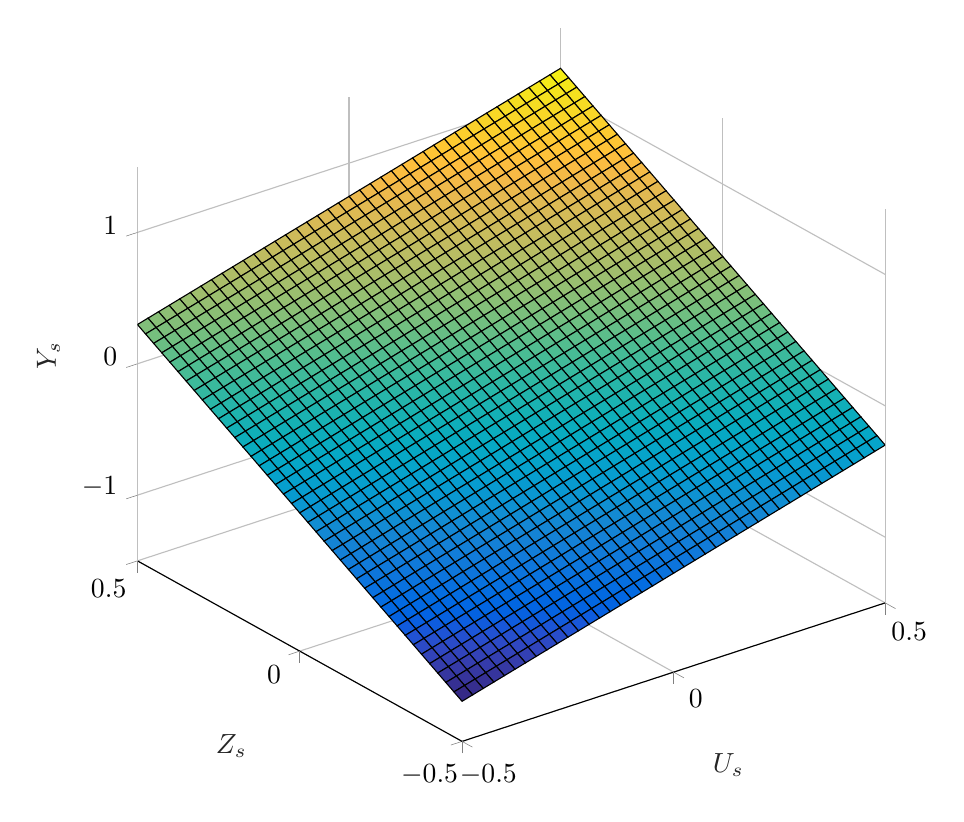
\begin{tikzpicture}

\begin{axis}[%
width=3.739in,
height=3.566in,
at={(0.66in,0.481in)},
scale only axis,
point meta min=-1.19475463603141,
point meta max=1.19475463603141,
xmin=-0.5,
xmax=0.5,
xtick={-0.5,0,0.5},
tick align=outside,
xlabel style={font=\color{white!15!black}},
xlabel={$U_s$},
ymin=-0.5,
ymax=0.5,
ytick={-0.5,0,0.5},
ylabel style={font=\color{white!15!black}},
ylabel={$Z_s$},
zmin=-1.5,
zmax=1.5,
zlabel style={font=\color{white!15!black}},
zlabel={$Y_s$},
view={-37.5}{30},
axis background/.style={fill=white},
axis x line*=bottom,
axis y line*=left,
axis z line*=left,
xmajorgrids,
ymajorgrids,
zmajorgrids,
colormap={mymap}{[1pt] rgb(0pt)=(0.2081,0.1663,0.5292); rgb(1pt)=(0.211624,0.189781,0.577676); rgb(2pt)=(0.212252,0.213771,0.626971); rgb(3pt)=(0.2081,0.2386,0.677086); rgb(4pt)=(0.195905,0.264457,0.7279); rgb(5pt)=(0.170729,0.291938,0.779248); rgb(6pt)=(0.125271,0.324243,0.830271); rgb(7pt)=(0.0591333,0.359833,0.868333); rgb(8pt)=(0.0116952,0.38751,0.881957); rgb(9pt)=(0.00595714,0.408614,0.882843); rgb(10pt)=(0.0165143,0.4266,0.878633); rgb(11pt)=(0.0328524,0.443043,0.871957); rgb(12pt)=(0.0498143,0.458571,0.864057); rgb(13pt)=(0.0629333,0.47369,0.855438); rgb(14pt)=(0.0722667,0.488667,0.8467); rgb(15pt)=(0.0779429,0.503986,0.838371); rgb(16pt)=(0.0793476,0.520024,0.831181); rgb(17pt)=(0.0749429,0.537543,0.826271); rgb(18pt)=(0.0640571,0.556986,0.823957); rgb(19pt)=(0.0487714,0.577224,0.822829); rgb(20pt)=(0.0343429,0.596581,0.819852); rgb(21pt)=(0.0265,0.6137,0.8135); rgb(22pt)=(0.0238905,0.628662,0.803762); rgb(23pt)=(0.0230905,0.641786,0.791267); rgb(24pt)=(0.0227714,0.653486,0.776757); rgb(25pt)=(0.0266619,0.664195,0.760719); rgb(26pt)=(0.0383714,0.674271,0.743552); rgb(27pt)=(0.0589714,0.683757,0.725386); rgb(28pt)=(0.0843,0.692833,0.706167); rgb(29pt)=(0.113295,0.7015,0.685857); rgb(30pt)=(0.145271,0.709757,0.664629); rgb(31pt)=(0.180133,0.717657,0.642433); rgb(32pt)=(0.217829,0.725043,0.619262); rgb(33pt)=(0.258643,0.731714,0.595429); rgb(34pt)=(0.302171,0.737605,0.571186); rgb(35pt)=(0.348167,0.742433,0.547267); rgb(36pt)=(0.395257,0.7459,0.524443); rgb(37pt)=(0.44201,0.748081,0.503314); rgb(38pt)=(0.487124,0.749062,0.483976); rgb(39pt)=(0.530029,0.749114,0.466114); rgb(40pt)=(0.570857,0.748519,0.44939); rgb(41pt)=(0.609852,0.747314,0.433686); rgb(42pt)=(0.6473,0.7456,0.4188); rgb(43pt)=(0.683419,0.743476,0.404433); rgb(44pt)=(0.71841,0.741133,0.390476); rgb(45pt)=(0.752486,0.7384,0.376814); rgb(46pt)=(0.785843,0.735567,0.363271); rgb(47pt)=(0.818505,0.732733,0.34979); rgb(48pt)=(0.850657,0.7299,0.336029); rgb(49pt)=(0.882433,0.727433,0.3217); rgb(50pt)=(0.913933,0.725786,0.306276); rgb(51pt)=(0.944957,0.726114,0.288643); rgb(52pt)=(0.973895,0.731395,0.266648); rgb(53pt)=(0.993771,0.745457,0.240348); rgb(54pt)=(0.999043,0.765314,0.216414); rgb(55pt)=(0.995533,0.786057,0.196652); rgb(56pt)=(0.988,0.8066,0.179367); rgb(57pt)=(0.978857,0.827143,0.163314); rgb(58pt)=(0.9697,0.848138,0.147452); rgb(59pt)=(0.962586,0.870514,0.1309); rgb(60pt)=(0.958871,0.8949,0.113243); rgb(61pt)=(0.959824,0.921833,0.0948381); rgb(62pt)=(0.9661,0.951443,0.0755333); rgb(63pt)=(0.9763,0.9831,0.0538)},
%colorbar
]

\addplot3[%
surf,
shader=flat corner, draw=black, z buffer=sort, colormap={mymap}{[1pt] rgb(0pt)=(0.2081,0.1663,0.5292); rgb(1pt)=(0.211624,0.189781,0.577676); rgb(2pt)=(0.212252,0.213771,0.626971); rgb(3pt)=(0.2081,0.2386,0.677086); rgb(4pt)=(0.195905,0.264457,0.7279); rgb(5pt)=(0.170729,0.291938,0.779248); rgb(6pt)=(0.125271,0.324243,0.830271); rgb(7pt)=(0.0591333,0.359833,0.868333); rgb(8pt)=(0.0116952,0.38751,0.881957); rgb(9pt)=(0.00595714,0.408614,0.882843); rgb(10pt)=(0.0165143,0.4266,0.878633); rgb(11pt)=(0.0328524,0.443043,0.871957); rgb(12pt)=(0.0498143,0.458571,0.864057); rgb(13pt)=(0.0629333,0.47369,0.855438); rgb(14pt)=(0.0722667,0.488667,0.8467); rgb(15pt)=(0.0779429,0.503986,0.838371); rgb(16pt)=(0.0793476,0.520024,0.831181); rgb(17pt)=(0.0749429,0.537543,0.826271); rgb(18pt)=(0.0640571,0.556986,0.823957); rgb(19pt)=(0.0487714,0.577224,0.822829); rgb(20pt)=(0.0343429,0.596581,0.819852); rgb(21pt)=(0.0265,0.6137,0.8135); rgb(22pt)=(0.0238905,0.628662,0.803762); rgb(23pt)=(0.0230905,0.641786,0.791267); rgb(24pt)=(0.0227714,0.653486,0.776757); rgb(25pt)=(0.0266619,0.664195,0.760719); rgb(26pt)=(0.0383714,0.674271,0.743552); rgb(27pt)=(0.0589714,0.683757,0.725386); rgb(28pt)=(0.0843,0.692833,0.706167); rgb(29pt)=(0.113295,0.7015,0.685857); rgb(30pt)=(0.145271,0.709757,0.664629); rgb(31pt)=(0.180133,0.717657,0.642433); rgb(32pt)=(0.217829,0.725043,0.619262); rgb(33pt)=(0.258643,0.731714,0.595429); rgb(34pt)=(0.302171,0.737605,0.571186); rgb(35pt)=(0.348167,0.742433,0.547267); rgb(36pt)=(0.395257,0.7459,0.524443); rgb(37pt)=(0.44201,0.748081,0.503314); rgb(38pt)=(0.487124,0.749062,0.483976); rgb(39pt)=(0.530029,0.749114,0.466114); rgb(40pt)=(0.570857,0.748519,0.44939); rgb(41pt)=(0.609852,0.747314,0.433686); rgb(42pt)=(0.6473,0.7456,0.4188); rgb(43pt)=(0.683419,0.743476,0.404433); rgb(44pt)=(0.71841,0.741133,0.390476); rgb(45pt)=(0.752486,0.7384,0.376814); rgb(46pt)=(0.785843,0.735567,0.363271); rgb(47pt)=(0.818505,0.732733,0.34979); rgb(48pt)=(0.850657,0.7299,0.336029); rgb(49pt)=(0.882433,0.727433,0.3217); rgb(50pt)=(0.913933,0.725786,0.306276); rgb(51pt)=(0.944957,0.726114,0.288643); rgb(52pt)=(0.973895,0.731395,0.266648); rgb(53pt)=(0.993771,0.745457,0.240348); rgb(54pt)=(0.999043,0.765314,0.216414); rgb(55pt)=(0.995533,0.786057,0.196652); rgb(56pt)=(0.988,0.8066,0.179367); rgb(57pt)=(0.978857,0.827143,0.163314); rgb(58pt)=(0.9697,0.848138,0.147452); rgb(59pt)=(0.962586,0.870514,0.1309); rgb(60pt)=(0.958871,0.8949,0.113243); rgb(61pt)=(0.959824,0.921833,0.0948381); rgb(62pt)=(0.9661,0.951443,0.0755333); rgb(63pt)=(0.9763,0.9831,0.0538)}, mesh/rows=41]
table[row sep=crcr, point meta=\thisrow{c}] {%
%
x	y	z	c\\
-0.5	-0.5	-1.19475463603141	-1.19475463603141\\
-0.5	-0.475	-1.15741361254645	-1.15741361254645\\
-0.5	-0.45	-1.12007258906149	-1.12007258906149\\
-0.5	-0.425	-1.08273156557656	-1.08273156557656\\
-0.5	-0.4	-1.0453905420916	-1.0453905420916\\
-0.5	-0.375	-1.00804951860663	-1.00804951860663\\
-0.5	-0.35	-0.970708495121707	-0.970708495121707\\
-0.5	-0.325	-0.933367471636742	-0.933367471636742\\
-0.5	-0.3	-0.896026448151778	-0.896026448151778\\
-0.5	-0.275	-0.858685424666838	-0.858685424666838\\
-0.5	-0.25	-0.821344401181891	-0.821344401181891\\
-0.5	-0.225	-0.784003377696925	-0.784003377696925\\
-0.5	-0.2	-0.746662354211964	-0.746662354211964\\
-0.5	-0.175	-0.709321330727038	-0.709321330727038\\
-0.5	-0.15	-0.671980307242073	-0.671980307242073\\
-0.5	-0.125	-0.634639283757112	-0.634639283757112\\
-0.5	-0.1	-0.597298260272184	-0.597298260272184\\
-0.5	-0.075	-0.559957236787219	-0.559957236787219\\
-0.5	-0.05	-0.522616213302278	-0.522616213302278\\
-0.5	-0.025	-0.485275189817313	-0.485275189817313\\
-0.5	0	-0.447934166332367	-0.447934166332367\\
-0.5	0.025	-0.410593142847422	-0.410593142847422\\
-0.5	0.05	-0.37325211936246	-0.37325211936246\\
-0.5	0.0750000000000001	-0.335911095877514	-0.335911095877514\\
-0.5	0.1	-0.298570072392568	-0.298570072392568\\
-0.5	0.125	-0.26122904890761	-0.26122904890761\\
-0.5	0.15	-0.223888025422661	-0.223888025422661\\
-0.5	0.175	-0.186547001937707	-0.186547001937707\\
-0.5	0.2	-0.149205978452753	-0.149205978452753\\
-0.5	0.225	-0.111864954967803	-0.111864954967803\\
-0.5	0.25	-0.0745239314828537	-0.0745239314828537\\
-0.5	0.275	-0.0371829079979023	-0.0371829079979023\\
-0.5	0.3	0.000158115487049622	0.000158115487049622\\
-0.5	0.325	0.0374991389720015	0.0374991389720015\\
-0.5	0.35	0.0748401624569533	0.0748401624569533\\
-0.5	0.375	0.112181185941905	0.112181185941905\\
-0.5	0.4	0.149522209426852	0.149522209426852\\
-0.5	0.425	0.186863232911806	0.186863232911806\\
-0.5	0.45	0.224204256396761	0.224204256396761\\
-0.5	0.475	0.261545279881714	0.261545279881714\\
-0.5	0.5	0.298886303366662	0.298886303366662\\
-0.475	-0.5	-1.17235792771474	-1.17235792771474\\
-0.475	-0.475	-1.13501690422986	-1.13501690422986\\
-0.475	-0.45	-1.0976758807449	-1.0976758807449\\
-0.475	-0.425	-1.06033485725993	-1.06033485725993\\
-0.475	-0.4	-1.02299383377497	-1.02299383377497\\
-0.475	-0.375	-0.985652810290044	-0.985652810290044\\
-0.475	-0.35	-0.948311786805072	-0.948311786805072\\
-0.475	-0.325	-0.910970763320112	-0.910970763320112\\
-0.475	-0.3	-0.87362973983517	-0.87362973983517\\
-0.475	-0.275	-0.836288716350225	-0.836288716350225\\
-0.475	-0.25	-0.798947692865258	-0.798947692865258\\
-0.475	-0.225	-0.761606669380297	-0.761606669380297\\
-0.475	-0.2	-0.724265645895368	-0.724265645895368\\
-0.475	-0.175	-0.686924622410408	-0.686924622410408\\
-0.475	-0.15	-0.649583598925443	-0.649583598925443\\
-0.475	-0.125	-0.612242575440521	-0.612242575440521\\
-0.475	-0.1	-0.574901551955556	-0.574901551955556\\
-0.475	-0.075	-0.53756052847061	-0.53756052847061\\
-0.475	-0.05	-0.500219504985644	-0.500219504985644\\
-0.475	-0.025	-0.4628784815007	-0.4628784815007\\
-0.475	0	-0.425537458015757	-0.425537458015757\\
-0.475	0.025	-0.388196434530792	-0.388196434530792\\
-0.475	0.05	-0.350855411045849	-0.350855411045849\\
-0.475	0.0750000000000001	-0.313514387560903	-0.313514387560903\\
-0.475	0.1	-0.27617336407594	-0.27617336407594\\
-0.475	0.125	-0.238832340590995	-0.238832340590995\\
-0.475	0.15	-0.201491317106041	-0.201491317106041\\
-0.475	0.175	-0.164150293621087	-0.164150293621087\\
-0.475	0.2	-0.126809270136137	-0.126809270136137\\
-0.475	0.225	-0.0894682466511879	-0.0894682466511879\\
-0.475	0.25	-0.0521272231662361	-0.0521272231662361\\
-0.475	0.275	-0.0147861996812843	-0.0147861996812843\\
-0.475	0.3	0.0225548238036676	0.0225548238036676\\
-0.475	0.325	0.0598958472886196	0.0598958472886196\\
-0.475	0.35	0.0972368707735709	0.0972368707735709\\
-0.475	0.375	0.134577894258523	0.134577894258523\\
-0.475	0.4	0.171918917743473	0.171918917743473\\
-0.475	0.425	0.209259941228427	0.209259941228427\\
-0.475	0.45	0.246600964713376	0.246600964713376\\
-0.475	0.475	0.283941988198326	0.283941988198326\\
-0.475	0.5	0.32128301168328	0.32128301168328\\
-0.45	-0.5	-1.14996121939816	-1.14996121939816\\
-0.45	-0.475	-1.11262019591319	-1.11262019591319\\
-0.45	-0.45	-1.07527917242827	-1.07527917242827\\
-0.45	-0.425	-1.0379381489433	-1.0379381489433\\
-0.45	-0.4	-1.00059712545835	-1.00059712545835\\
-0.45	-0.375	-0.963256101973411	-0.963256101973411\\
-0.45	-0.35	-0.925915078488445	-0.925915078488445\\
-0.45	-0.325	-0.888574055003485	-0.888574055003485\\
-0.45	-0.3	-0.851233031518557	-0.851233031518557\\
-0.45	-0.275	-0.813892008033595	-0.813892008033595\\
-0.45	-0.25	-0.776550984548629	-0.776550984548629\\
-0.45	-0.225	-0.739209961063704	-0.739209961063704\\
-0.45	-0.2	-0.701868937578742	-0.701868937578742\\
-0.45	-0.175	-0.664527914093779	-0.664527914093779\\
-0.45	-0.15	-0.627186890608855	-0.627186890608855\\
-0.45	-0.125	-0.58984586712389	-0.58984586712389\\
-0.45	-0.1	-0.552504843638926	-0.552504843638926\\
-0.45	-0.075	-0.515163820153982	-0.515163820153982\\
-0.45	-0.05	-0.477822796669036	-0.477822796669036\\
-0.45	-0.025	-0.44048177318409	-0.44048177318409\\
-0.45	0	-0.403140749699126	-0.403140749699126\\
-0.45	0.025	-0.365799726214181	-0.365799726214181\\
-0.45	0.05	-0.328458702729238	-0.328458702729238\\
-0.45	0.0750000000000001	-0.291117679244273	-0.291117679244273\\
-0.45	0.1	-0.25377665575933	-0.25377665575933\\
-0.45	0.125	-0.216435632274375	-0.216435632274375\\
-0.45	0.15	-0.17909460878942	-0.17909460878942\\
-0.45	0.175	-0.141753585304472	-0.141753585304472\\
-0.45	0.2	-0.10441256181952	-0.10441256181952\\
-0.45	0.225	-0.0670715383345678	-0.0670715383345678\\
-0.45	0.25	-0.0297305148496169	-0.0297305148496169\\
-0.45	0.275	0.00761050863533476	0.00761050863533476\\
-0.45	0.3	0.0449515321202862	0.0449515321202862\\
-0.45	0.325	0.0822925556052398	0.0822925556052398\\
-0.45	0.35	0.119633579090189	0.119633579090189\\
-0.45	0.375	0.156974602575139	0.156974602575139\\
-0.45	0.4	0.194315626060092	0.194315626060092\\
-0.45	0.425	0.231656649545047	0.231656649545047\\
-0.45	0.45	0.268997673029992	0.268997673029992\\
-0.45	0.475	0.306338696514954	0.306338696514954\\
-0.45	0.5	0.343679719999899	0.343679719999899\\
-0.425	-0.5	-1.12756451108156	-1.12756451108156\\
-0.425	-0.475	-1.09022348759658	-1.09022348759658\\
-0.425	-0.45	-1.05288246411163	-1.05288246411163\\
-0.425	-0.425	-1.01554144062669	-1.01554144062669\\
-0.425	-0.4	-0.978200417141748	-0.978200417141748\\
-0.425	-0.375	-0.940859393656779	-0.940859393656779\\
-0.425	-0.35	-0.903518370171817	-0.903518370171817\\
-0.425	-0.325	-0.866177346686892	-0.866177346686892\\
-0.425	-0.3	-0.82883632320193	-0.82883632320193\\
-0.425	-0.275	-0.791495299716968	-0.791495299716968\\
-0.425	-0.25	-0.754154276232038	-0.754154276232038\\
-0.425	-0.225	-0.716813252747075	-0.716813252747075\\
-0.425	-0.2	-0.679472229262112	-0.679472229262112\\
-0.425	-0.175	-0.642131205777187	-0.642131205777187\\
-0.425	-0.15	-0.604790182292222	-0.604790182292222\\
-0.425	-0.125	-0.567449158807258	-0.567449158807258\\
-0.425	-0.1	-0.530108135322313	-0.530108135322313\\
-0.425	-0.075	-0.49276711183737	-0.49276711183737\\
-0.425	-0.05	-0.455426088352424	-0.455426088352424\\
-0.425	-0.025	-0.41808506486746	-0.41808506486746\\
-0.425	0	-0.380744041382516	-0.380744041382516\\
-0.425	0.025	-0.343403017897563	-0.343403017897563\\
-0.425	0.05	-0.306061994412608	-0.306061994412608\\
-0.425	0.0750000000000001	-0.268720970927662	-0.268720970927662\\
-0.425	0.1	-0.231379947442709	-0.231379947442709\\
-0.425	0.125	-0.194038923957754	-0.194038923957754\\
-0.425	0.15	-0.1566979004728	-0.1566979004728\\
-0.425	0.175	-0.119356876987853	-0.119356876987853\\
-0.425	0.2	-0.0820158535029017	-0.0820158535029017\\
-0.425	0.225	-0.0446748300179497	-0.0446748300179497\\
-0.425	0.25	-0.00733380653299909	-0.00733380653299909\\
-0.425	0.275	0.0300072169519527	0.0300072169519527\\
-0.425	0.3	0.0673482404369048	0.0673482404369048\\
-0.425	0.325	0.104689263921855	0.104689263921855\\
-0.425	0.35	0.142030287406805	0.142030287406805\\
-0.425	0.375	0.179371310891759	0.179371310891759\\
-0.425	0.4	0.216712334376713	0.216712334376713\\
-0.425	0.425	0.254053357861663	0.254053357861663\\
-0.425	0.45	0.291394381346622	0.291394381346622\\
-0.425	0.475	0.328735404831566	0.328735404831566\\
-0.425	0.5	0.366076428316511	0.366076428316511\\
-0.4	-0.5	-1.10516780276489	-1.10516780276489\\
-0.4	-0.475	-1.06782677927997	-1.06782677927997\\
-0.4	-0.45	-1.03048575579503	-1.03048575579503\\
-0.4	-0.425	-0.993144732310077	-0.993144732310077\\
-0.4	-0.4	-0.955803708825115	-0.955803708825115\\
-0.4	-0.375	-0.91846268534015	-0.91846268534015\\
-0.4	-0.35	-0.881121661855223	-0.881121661855223\\
-0.4	-0.325	-0.843780638370264	-0.843780638370264\\
-0.4	-0.3	-0.806439614885298	-0.806439614885298\\
-0.4	-0.275	-0.76909859140037	-0.76909859140037\\
-0.4	-0.25	-0.731757567915406	-0.731757567915406\\
-0.4	-0.225	-0.694416544430446	-0.694416544430446\\
-0.4	-0.2	-0.65707552094552	-0.65707552094552\\
-0.4	-0.175	-0.619734497460555	-0.619734497460555\\
-0.4	-0.15	-0.58239347397559	-0.58239347397559\\
-0.4	-0.125	-0.545052450490658	-0.545052450490658\\
-0.4	-0.1	-0.507711427005703	-0.507711427005703\\
-0.4	-0.075	-0.470370403520757	-0.470370403520757\\
-0.4	-0.05	-0.433029380035796	-0.433029380035796\\
-0.4	-0.025	-0.395688356550849	-0.395688356550849\\
-0.4	0	-0.358347333065896	-0.358347333065896\\
-0.4	0.025	-0.321006309580941	-0.321006309580941\\
-0.4	0.05	-0.283665286095997	-0.283665286095997\\
-0.4	0.0750000000000001	-0.246324262611043	-0.246324262611043\\
-0.4	0.1	-0.208983239126088	-0.208983239126088\\
-0.4	0.125	-0.171642215641134	-0.171642215641134\\
-0.4	0.15	-0.134301192156187	-0.134301192156187\\
-0.4	0.175	-0.0969601686712352	-0.0969601686712352\\
-0.4	0.2	-0.0596191451862834	-0.0596191451862834\\
-0.4	0.225	-0.0222781217013318	-0.0222781217013318\\
-0.4	0.25	0.0150629017836199	0.0150629017836199\\
-0.4	0.275	0.0524039252685708	0.0524039252685708\\
-0.4	0.3	0.0897449487535214	0.0897449487535214\\
-0.4	0.325	0.127085972238473	0.127085972238473\\
-0.4	0.35	0.164426995723424	0.164426995723424\\
-0.4	0.375	0.201768019208379	0.201768019208379\\
-0.4	0.4	0.239109042693328	0.239109042693328\\
-0.4	0.425	0.276450066178287	0.276450066178287\\
-0.4	0.45	0.313791089663232	0.313791089663232\\
-0.4	0.475	0.351132113148177	0.351132113148177\\
-0.4	0.5	0.388473136633142	0.388473136633142\\
-0.375	-0.5	-1.0827710944483	-1.0827710944483\\
-0.375	-0.475	-1.04543007096334	-1.04543007096334\\
-0.375	-0.45	-1.00808904747841	-1.00808904747841\\
-0.375	-0.425	-0.970748023993449	-0.970748023993449\\
-0.375	-0.4	-0.933407000508485	-0.933407000508485\\
-0.375	-0.375	-0.89606597702356	-0.89606597702356\\
-0.375	-0.35	-0.858724953538596	-0.858724953538596\\
-0.375	-0.325	-0.821383930053633	-0.821383930053633\\
-0.375	-0.3	-0.784042906568705	-0.784042906568705\\
-0.375	-0.275	-0.746701883083745	-0.746701883083745\\
-0.375	-0.25	-0.709360859598781	-0.709360859598781\\
-0.375	-0.225	-0.672019836113851	-0.672019836113851\\
-0.375	-0.2	-0.634678812628885	-0.634678812628885\\
-0.375	-0.175	-0.597337789143927	-0.597337789143927\\
-0.375	-0.15	-0.559996765658999	-0.559996765658999\\
-0.375	-0.125	-0.522655742174036	-0.522655742174036\\
-0.375	-0.1	-0.485314718689082	-0.485314718689082\\
-0.375	-0.075	-0.447973695204128	-0.447973695204128\\
-0.375	-0.05	-0.410632671719184	-0.410632671719184\\
-0.375	-0.025	-0.37329164823422	-0.37329164823422\\
-0.375	0	-0.335950624749276	-0.335950624749276\\
-0.375	0.025	-0.298609601264331	-0.298609601264331\\
-0.375	0.05	-0.261268577779376	-0.261268577779376\\
-0.375	0.0750000000000001	-0.223927554294422	-0.223927554294422\\
-0.375	0.1	-0.186586530809468	-0.186586530809468\\
-0.375	0.125	-0.149245507324519	-0.149245507324519\\
-0.375	0.15	-0.111904483839566	-0.111904483839566\\
-0.375	0.175	-0.0745634603546153	-0.0745634603546153\\
-0.375	0.2	-0.0372224368696646	-0.0372224368696646\\
-0.375	0.225	0.000118586615287216	0.000118586615287216\\
-0.375	0.25	0.0374596101002377	0.0374596101002377\\
-0.375	0.275	0.07480063358519	0.07480063358519\\
-0.375	0.3	0.112141657070142	0.112141657070142\\
-0.375	0.325	0.149482680555091	0.149482680555091\\
-0.375	0.35	0.186823704040044	0.186823704040044\\
-0.375	0.375	0.224164727524999	0.224164727524999\\
-0.375	0.4	0.261505751009943	0.261505751009943\\
-0.375	0.425	0.298846774494898	0.298846774494898\\
-0.375	0.45	0.336187797979843	0.336187797979843\\
-0.375	0.475	0.373528821464807	0.373528821464807\\
-0.375	0.5	0.41086984494975	0.41086984494975\\
-0.35	-0.5	-1.06037438613167	-1.06037438613167\\
-0.35	-0.475	-1.02303336264675	-1.02303336264675\\
-0.35	-0.45	-0.985692339161782	-0.985692339161782\\
-0.35	-0.425	-0.948351315676821	-0.948351315676821\\
-0.35	-0.4	-0.911010292191893	-0.911010292191893\\
-0.35	-0.375	-0.873669268706928	-0.873669268706928\\
-0.35	-0.35	-0.836328245221966	-0.836328245221966\\
-0.35	-0.325	-0.79898722173704	-0.79898722173704\\
-0.35	-0.3	-0.761646198252075	-0.761646198252075\\
-0.35	-0.275	-0.724305174767114	-0.724305174767114\\
-0.35	-0.25	-0.686964151282185	-0.686964151282185\\
-0.35	-0.225	-0.649623127797224	-0.649623127797224\\
-0.35	-0.2	-0.61228210431226	-0.61228210431226\\
-0.35	-0.175	-0.574941080827337	-0.574941080827337\\
-0.35	-0.15	-0.53760005734237	-0.53760005734237\\
-0.35	-0.125	-0.500259033857406	-0.500259033857406\\
-0.35	-0.1	-0.462918010372463	-0.462918010372463\\
-0.35	-0.075	-0.425576986887519	-0.425576986887519\\
-0.35	-0.05	-0.388235963402552	-0.388235963402552\\
-0.35	-0.025	-0.350894939917608	-0.350894939917608\\
-0.35	0	-0.313553916432665	-0.313553916432665\\
-0.35	0.025	-0.276212892947701	-0.276212892947701\\
-0.35	0.05	-0.238871869462756	-0.238871869462756\\
-0.35	0.0750000000000001	-0.201530845977802	-0.201530845977802\\
-0.35	0.1	-0.164189822492848	-0.164189822492848\\
-0.35	0.125	-0.126848799007899	-0.126848799007899\\
-0.35	0.15	-0.0895077755229489	-0.0895077755229489\\
-0.35	0.175	-0.0521667520379975	-0.0521667520379975\\
-0.35	0.2	-0.0148257285530455	-0.0148257285530455\\
-0.35	0.225	0.0225152949319062	0.0225152949319062\\
-0.35	0.25	0.0598563184168573	0.0598563184168573\\
-0.35	0.275	0.0971973419018076	0.0971973419018076\\
-0.35	0.3	0.134538365386762	0.134538365386762\\
-0.35	0.325	0.171879388871711	0.171879388871711\\
-0.35	0.35	0.209220412356666	0.209220412356666\\
-0.35	0.375	0.246561435841619	0.246561435841619\\
-0.35	0.4	0.283902459326564	0.283902459326564\\
-0.35	0.425	0.321243482811517	0.321243482811517\\
-0.35	0.45	0.358584506296473	0.358584506296473\\
-0.35	0.475	0.395925529781418	0.395925529781418\\
-0.35	0.5	0.43326655326638	0.43326655326638\\
-0.325	-0.5	-1.03797767781508	-1.03797767781508\\
-0.325	-0.475	-1.00063665433012	-1.00063665433012\\
-0.325	-0.45	-0.963295630845151	-0.963295630845151\\
-0.325	-0.425	-0.92595460736023	-0.92595460736023\\
-0.325	-0.4	-0.888613583875265	-0.888613583875265\\
-0.325	-0.375	-0.851272560390302	-0.851272560390302\\
-0.325	-0.35	-0.813931536905375	-0.813931536905375\\
-0.325	-0.325	-0.776590513420411	-0.776590513420411\\
-0.325	-0.3	-0.739249489935445	-0.739249489935445\\
-0.325	-0.275	-0.70190846645052	-0.70190846645052\\
-0.325	-0.25	-0.664567442965561	-0.664567442965561\\
-0.325	-0.225	-0.627226419480596	-0.627226419480596\\
-0.325	-0.2	-0.589885395995671	-0.589885395995671\\
-0.325	-0.175	-0.552544372510705	-0.552544372510705\\
-0.325	-0.15	-0.51520334902574	-0.51520334902574\\
-0.325	-0.125	-0.477862325540797	-0.477862325540797\\
-0.325	-0.1	-0.440521302055853	-0.440521302055853\\
-0.325	-0.075	-0.403180278570888	-0.403180278570888\\
-0.325	-0.05	-0.365839255085942	-0.365839255085942\\
-0.325	-0.025	-0.328498231600999	-0.328498231600999\\
-0.325	0	-0.291157208116035	-0.291157208116035\\
-0.325	0.025	-0.253816184631091	-0.253816184631091\\
-0.325	0.05	-0.216475161146136	-0.216475161146136\\
-0.325	0.0750000000000001	-0.179134137661183	-0.179134137661183\\
-0.325	0.1	-0.141793114176237	-0.141793114176237\\
-0.325	0.125	-0.104452090691283	-0.104452090691283\\
-0.325	0.15	-0.06711106720633	-0.06711106720633\\
-0.325	0.175	-0.0297700437213794	-0.0297700437213794\\
-0.325	0.2	0.00757097976357238	0.00757097976357238\\
-0.325	0.225	0.0449120032485242	0.0449120032485242\\
-0.325	0.25	0.0822530267334738	0.0822530267334738\\
-0.325	0.275	0.119594050218428	0.119594050218428\\
-0.325	0.3	0.156935073703377	0.156935073703377\\
-0.325	0.325	0.194276097188332	0.194276097188332\\
-0.325	0.35	0.231617120673285	0.231617120673285\\
-0.325	0.375	0.268958144158229	0.268958144158229\\
-0.325	0.4	0.306299167643183	0.306299167643183\\
-0.325	0.425	0.343640191128138	0.343640191128138\\
-0.325	0.45	0.380981214613083	0.380981214613083\\
-0.325	0.475	0.418322238098047	0.418322238098047\\
-0.325	0.5	0.455663261582992	0.455663261582992\\
-0.3	-0.5	-1.01558096949846	-1.01558096949846\\
-0.3	-0.475	-0.978239946013487	-0.978239946013487\\
-0.3	-0.45	-0.940898922528563	-0.940898922528563\\
-0.3	-0.425	-0.9035578990436	-0.9035578990436\\
-0.3	-0.4	-0.866216875558636	-0.866216875558636\\
-0.3	-0.375	-0.82887585207371	-0.82887585207371\\
-0.3	-0.35	-0.791534828588743	-0.791534828588743\\
-0.3	-0.325	-0.754193805103781	-0.754193805103781\\
-0.3	-0.3	-0.716852781618853	-0.716852781618853\\
-0.3	-0.275	-0.679511758133893	-0.679511758133893\\
-0.3	-0.25	-0.642170734648927	-0.642170734648927\\
-0.3	-0.225	-0.604829711163999	-0.604829711163999\\
-0.3	-0.2	-0.567488687679038	-0.567488687679038\\
-0.3	-0.175	-0.530147664194076	-0.530147664194076\\
-0.3	-0.15	-0.49280664070913	-0.49280664070913\\
-0.3	-0.125	-0.455465617224186	-0.455465617224186\\
-0.3	-0.1	-0.418124593739222	-0.418124593739222\\
-0.3	-0.075	-0.380783570254278	-0.380783570254278\\
-0.3	-0.05	-0.343442546769324	-0.343442546769324\\
-0.3	-0.025	-0.306101523284369	-0.306101523284369\\
-0.3	0	-0.268760499799425	-0.268760499799425\\
-0.3	0.025	-0.231419476314469	-0.231419476314469\\
-0.3	0.05	-0.194078452829516	-0.194078452829516\\
-0.3	0.0750000000000001	-0.156737429344561	-0.156737429344561\\
-0.3	0.1	-0.119396405859614	-0.119396405859614\\
-0.3	0.125	-0.0820553823746629	-0.0820553823746629\\
-0.3	0.15	-0.044714358889711	-0.044714358889711\\
-0.3	0.175	-0.00737333540476034	-0.00737333540476034\\
-0.3	0.2	0.0299676880801915	0.0299676880801915\\
-0.3	0.225	0.0673087115651432	0.0673087115651432\\
-0.3	0.25	0.104649735050094	0.104649735050094\\
-0.3	0.275	0.141990758535044	0.141990758535044\\
-0.3	0.3	0.179331782019998	0.179331782019998\\
-0.3	0.325	0.216672805504951	0.216672805504951\\
-0.3	0.35	0.254013828989897	0.254013828989897\\
-0.3	0.375	0.291354852474858	0.291354852474858\\
-0.3	0.4	0.328695875959804	0.328695875959804\\
-0.3	0.425	0.366036899444749	0.366036899444749\\
-0.3	0.45	0.403377922929714	0.403377922929714\\
-0.3	0.475	0.440718946414659	0.440718946414659\\
-0.3	0.5	0.478059969899603	0.478059969899603\\
-0.275	-0.5	-0.993184261181821	-0.993184261181821\\
-0.275	-0.475	-0.955843237696892	-0.955843237696892\\
-0.275	-0.45	-0.918502214211932	-0.918502214211932\\
-0.275	-0.425	-0.881161190726969	-0.881161190726969\\
-0.275	-0.4	-0.843820167242041	-0.843820167242041\\
-0.275	-0.375	-0.806479143757079	-0.806479143757079\\
-0.275	-0.35	-0.769138120272114	-0.769138120272114\\
-0.275	-0.325	-0.731797096787189	-0.731797096787189\\
-0.275	-0.3	-0.694456073302225	-0.694456073302225\\
-0.275	-0.275	-0.657115049817262	-0.657115049817262\\
-0.275	-0.25	-0.619774026332334	-0.619774026332334\\
-0.275	-0.225	-0.582433002847372	-0.582433002847372\\
-0.275	-0.2	-0.545091979362416	-0.545091979362416\\
-0.275	-0.175	-0.507750955877464	-0.507750955877464\\
-0.275	-0.15	-0.470409932392519	-0.470409932392519\\
-0.275	-0.125	-0.433068908907557	-0.433068908907557\\
-0.275	-0.1	-0.395727885422611	-0.395727885422611\\
-0.275	-0.075	-0.358386861937656	-0.358386861937656\\
-0.275	-0.05	-0.321045838452704	-0.321045838452704\\
-0.275	-0.025	-0.283704814967758	-0.283704814967758\\
-0.275	0	-0.246363791482804	-0.246363791482804\\
-0.275	0.025	-0.20902276799785	-0.20902276799785\\
-0.275	0.05	-0.171681744512895	-0.171681744512895\\
-0.275	0.0750000000000001	-0.134340721027946	-0.134340721027946\\
-0.275	0.1	-0.0969996975429965	-0.0969996975429965\\
-0.275	0.125	-0.059658674058045	-0.059658674058045\\
-0.275	0.15	-0.0223176505730938	-0.0223176505730938\\
-0.275	0.175	0.0150233729118575	0.0150233729118575\\
-0.275	0.2	0.0523643963968093	0.0523643963968093\\
-0.275	0.225	0.0897054198817597	0.0897054198817597\\
-0.275	0.25	0.127046443366714	0.127046443366714\\
-0.275	0.275	0.164387466851664	0.164387466851664\\
-0.275	0.3	0.201728490336618	0.201728490336618\\
-0.275	0.325	0.239069513821562	0.239069513821562\\
-0.275	0.35	0.276410537306526	0.276410537306526\\
-0.275	0.375	0.31375156079147	0.31375156079147\\
-0.275	0.4	0.351092584276416	0.351092584276416\\
-0.275	0.425	0.38843360776138	0.38843360776138\\
-0.275	0.45	0.425774631246323	0.425774631246323\\
-0.275	0.475	0.463115654731268	0.463115654731268\\
-0.275	0.5	0.500456678216231	0.500456678216231\\
-0.25	-0.5	-0.970787552865228	-0.970787552865228\\
-0.25	-0.475	-0.933446529380265	-0.933446529380265\\
-0.25	-0.45	-0.8961055058953	-0.8961055058953\\
-0.25	-0.425	-0.858764482410375	-0.858764482410375\\
-0.25	-0.4	-0.821423458925412	-0.821423458925412\\
-0.25	-0.375	-0.784082435440451	-0.784082435440451\\
-0.25	-0.35	-0.746741411955521	-0.746741411955521\\
-0.25	-0.325	-0.709400388470558	-0.709400388470558\\
-0.25	-0.3	-0.672059364985596	-0.672059364985596\\
-0.25	-0.275	-0.634718341500633	-0.634718341500633\\
-0.25	-0.25	-0.597377318015703	-0.597377318015703\\
-0.25	-0.225	-0.560036294530743	-0.560036294530743\\
-0.25	-0.2	-0.522695271045799	-0.522695271045799\\
-0.25	-0.175	-0.485354247560853	-0.485354247560853\\
-0.25	-0.15	-0.448013224075889	-0.448013224075889\\
-0.25	-0.125	-0.410672200590946	-0.410672200590946\\
-0.25	-0.1	-0.373331177105982	-0.373331177105982\\
-0.25	-0.075	-0.335990153621036	-0.335990153621036\\
-0.25	-0.05	-0.298649130136092	-0.298649130136092\\
-0.25	-0.025	-0.261308106651139	-0.261308106651139\\
-0.25	0	-0.223967083166183	-0.223967083166183\\
-0.25	0.025	-0.18662605968123	-0.18662605968123\\
-0.25	0.05	-0.149285036196284	-0.149285036196284\\
-0.25	0.0750000000000001	-0.11194401271133	-0.11194401271133\\
-0.25	0.1	-0.0746029892263765	-0.0746029892263765\\
-0.25	0.125	-0.0372619657414269	-0.0372619657414269\\
-0.25	0.15	7.90577435248108e-05	7.90577435248108e-05\\
-0.25	0.175	0.0374200812284766	0.0374200812284766\\
-0.25	0.2	0.0747611047134289	0.0747611047134289\\
-0.25	0.225	0.11210212819838	0.11210212819838\\
-0.25	0.25	0.149443151683331	0.149443151683331\\
-0.25	0.275	0.186784175168283	0.186784175168283\\
-0.25	0.3	0.224125198653238	0.224125198653238\\
-0.25	0.325	0.261466222138183	0.261466222138183\\
-0.25	0.35	0.298807245623137	0.298807245623137\\
-0.25	0.375	0.336148269108081	0.336148269108081\\
-0.25	0.4	0.373489292593044	0.373489292593044\\
-0.25	0.425	0.410830316077991	0.410830316077991\\
-0.25	0.45	0.448171339562935	0.448171339562935\\
-0.25	0.475	0.485512363047897	0.485512363047897\\
-0.25	0.5	0.522853386532843	0.522853386532843\\
-0.225	-0.5	-0.948390844548601	-0.948390844548601\\
-0.225	-0.475	-0.911049821063639	-0.911049821063639\\
-0.225	-0.45	-0.873708797578709	-0.873708797578709\\
-0.225	-0.425	-0.836367774093746	-0.836367774093746\\
-0.225	-0.4	-0.799026750608781	-0.799026750608781\\
-0.225	-0.375	-0.761685727123855	-0.761685727123855\\
-0.225	-0.35	-0.724344703638894	-0.724344703638894\\
-0.225	-0.325	-0.687003680153931	-0.687003680153931\\
-0.225	-0.3	-0.649662656668966	-0.649662656668966\\
-0.225	-0.275	-0.61232163318404	-0.61232163318404\\
-0.225	-0.25	-0.574980609699078	-0.574980609699078\\
-0.225	-0.225	-0.537639586214134	-0.537639586214134\\
-0.225	-0.2	-0.500298562729176	-0.500298562729176\\
-0.225	-0.175	-0.462957539244223	-0.462957539244223\\
-0.225	-0.15	-0.425616515759279	-0.425616515759279\\
-0.225	-0.125	-0.388275492274315	-0.388275492274315\\
-0.225	-0.1	-0.350934468789371	-0.350934468789371\\
-0.225	-0.075	-0.313593445304427	-0.313593445304427\\
-0.225	-0.05	-0.276252421819463	-0.276252421819463\\
-0.225	-0.025	-0.238911398334518	-0.238911398334518\\
-0.225	0	-0.201570374849563	-0.201570374849563\\
-0.225	0.025	-0.164229351364614	-0.164229351364614\\
-0.225	0.05	-0.126888327879665	-0.126888327879665\\
-0.225	0.0750000000000001	-0.0895473043947101	-0.0895473043947101\\
-0.225	0.1	-0.0522062809097598	-0.0522062809097598\\
-0.225	0.125	-0.0148652574248079	-0.0148652574248079\\
-0.225	0.15	0.0224757660601431	0.0224757660601431\\
-0.225	0.175	0.0598167895450947	0.0598167895450947\\
-0.225	0.2	0.0971578130300461	0.0971578130300461\\
-0.225	0.225	0.134498836514998	0.134498836514998\\
-0.225	0.25	0.17183985999995	0.17183985999995\\
-0.225	0.275	0.209180883484905	0.209180883484905\\
-0.225	0.3	0.246521906969849	0.246521906969849\\
-0.225	0.325	0.283862930454803	0.283862930454803\\
-0.225	0.35	0.321203953939748	0.321203953939748\\
-0.225	0.375	0.358544977424711	0.358544977424711\\
-0.225	0.4	0.395886000909657	0.395886000909657\\
-0.225	0.425	0.433227024394609	0.433227024394609\\
-0.225	0.45	0.470568047879566	0.470568047879566\\
-0.225	0.475	0.507909071364508	0.507909071364508\\
-0.225	0.5	0.545250094849467	0.545250094849467\\
-0.2	-0.5	-0.92599413623197	-0.92599413623197\\
-0.2	-0.475	-0.888653112747044	-0.888653112747044\\
-0.2	-0.45	-0.851312089262078	-0.851312089262078\\
-0.2	-0.425	-0.813971065777114	-0.813971065777114\\
-0.2	-0.4	-0.776630042292155	-0.776630042292155\\
-0.2	-0.375	-0.739289018807224	-0.739289018807224\\
-0.2	-0.35	-0.701947995322266	-0.701947995322266\\
-0.2	-0.325	-0.664606971837302	-0.664606971837302\\
-0.2	-0.3	-0.627265948352375	-0.627265948352375\\
-0.2	-0.275	-0.589924924867414	-0.589924924867414\\
-0.2	-0.25	-0.552583901382444	-0.552583901382444\\
-0.2	-0.225	-0.5152428778975	-0.5152428778975\\
-0.2	-0.2	-0.477901854412557	-0.477901854412557\\
-0.2	-0.175	-0.440560830927614	-0.440560830927614\\
-0.2	-0.15	-0.403219807442649	-0.403219807442649\\
-0.2	-0.125	-0.365878783957703	-0.365878783957703\\
-0.2	-0.1	-0.32853776047276	-0.32853776047276\\
-0.2	-0.075	-0.291196736987795	-0.291196736987795\\
-0.2	-0.05	-0.253855713502851	-0.253855713502851\\
-0.2	-0.025	-0.216514690017897	-0.216514690017897\\
-0.2	0	-0.179173666532943	-0.179173666532943\\
-0.2	0.025	-0.141832643047998	-0.141832643047998\\
-0.2	0.05	-0.104491619563044	-0.104491619563044\\
-0.2	0.0750000000000001	-0.0671505960780924	-0.0671505960780924\\
-0.2	0.1	-0.0298095725931413	-0.0298095725931413\\
-0.2	0.125	0.00753145089181056	0.00753145089181056\\
-0.2	0.15	0.044872474376762	0.044872474376762\\
-0.2	0.175	0.0822134978617122	0.0822134978617122\\
-0.2	0.2	0.119554521346666	0.119554521346666\\
-0.2	0.225	0.156895544831616	0.156895544831616\\
-0.2	0.25	0.19423656831657	0.19423656831657\\
-0.2	0.275	0.231577591801514	0.231577591801514\\
-0.2	0.3	0.26891861528647	0.26891861528647\\
-0.2	0.325	0.306259638771414	0.306259638771414\\
-0.2	0.35	0.343600662256378	0.343600662256378\\
-0.2	0.375	0.380941685741323	0.380941685741323\\
-0.2	0.4	0.418282709226286	0.418282709226286\\
-0.2	0.425	0.45562373271123	0.45562373271123\\
-0.2	0.45	0.492964756196175	0.492964756196175\\
-0.2	0.475	0.530305779681141	0.530305779681141\\
-0.2	0.5	0.567646803166082	0.567646803166082\\
-0.175	-0.5	-0.903597427915353	-0.903597427915353\\
-0.175	-0.475	-0.866256404430412	-0.866256404430412\\
-0.175	-0.45	-0.828915380945451	-0.828915380945451\\
-0.175	-0.425	-0.791574357460487	-0.791574357460487\\
-0.175	-0.4	-0.754233333975562	-0.754233333975562\\
-0.175	-0.375	-0.716892310490596	-0.716892310490596\\
-0.175	-0.35	-0.679551287005636	-0.679551287005636\\
-0.175	-0.325	-0.642210263520706	-0.642210263520706\\
-0.175	-0.3	-0.604869240035743	-0.604869240035743\\
-0.175	-0.275	-0.567528216550783	-0.567528216550783\\
-0.175	-0.25	-0.530187193065837	-0.530187193065837\\
-0.175	-0.225	-0.492846169580891	-0.492846169580891\\
-0.175	-0.2	-0.455505146095946	-0.455505146095946\\
-0.175	-0.175	-0.418164122610983	-0.418164122610983\\
-0.175	-0.15	-0.380823099126037	-0.380823099126037\\
-0.175	-0.125	-0.343482075641093	-0.343482075641093\\
-0.175	-0.1	-0.30614105215613	-0.30614105215613\\
-0.175	-0.075	-0.268800028671187	-0.268800028671187\\
-0.175	-0.05	-0.231459005186232	-0.231459005186232\\
-0.175	-0.025	-0.194117981701276	-0.194117981701276\\
-0.175	0	-0.156776958216333	-0.156776958216333\\
-0.175	0.025	-0.119435934731378	-0.119435934731378\\
-0.175	0.05	-0.0820949112464239	-0.0820949112464239\\
-0.175	0.0750000000000001	-0.0447538877614744	-0.0447538877614744\\
-0.175	0.1	-0.00741286427652275	-0.00741286427652275\\
-0.175	0.125	0.0299281592084287	0.0299281592084287\\
-0.175	0.15	0.0672691826933809	0.0672691826933809\\
-0.175	0.175	0.104610206178333	0.104610206178333\\
-0.175	0.2	0.141951229663283	0.141951229663283\\
-0.175	0.225	0.179292253148237	0.179292253148237\\
-0.175	0.25	0.21663327663319	0.21663327663319\\
-0.175	0.275	0.253974300118136	0.253974300118136\\
-0.175	0.3	0.29131532360309	0.29131532360309\\
-0.175	0.325	0.328656347088043	0.328656347088043\\
-0.175	0.35	0.365997370572989	0.365997370572989\\
-0.175	0.375	0.403338394057952	0.403338394057952\\
-0.175	0.4	0.440679417542897	0.440679417542897\\
-0.175	0.425	0.478020441027841	0.478020441027841\\
-0.175	0.45	0.515361464512805	0.515361464512805\\
-0.175	0.475	0.55270248799775	0.55270248799775\\
-0.175	0.5	0.590043511482713	0.590043511482713\\
-0.15	-0.5	-0.881200719598749	-0.881200719598749\\
-0.15	-0.475	-0.843859696113784	-0.843859696113784\\
-0.15	-0.45	-0.80651867262882	-0.80651867262882\\
-0.15	-0.425	-0.769177649143892	-0.769177649143892\\
-0.15	-0.4	-0.731836625658929	-0.731836625658929\\
-0.15	-0.375	-0.69449560217397	-0.69449560217397\\
-0.15	-0.35	-0.657154578689042	-0.657154578689042\\
-0.15	-0.325	-0.619813555204081	-0.619813555204081\\
-0.15	-0.3	-0.582472531719115	-0.582472531719115\\
-0.15	-0.275	-0.54513150823418	-0.54513150823418\\
-0.15	-0.25	-0.507790484749223	-0.507790484749223\\
-0.15	-0.225	-0.470449461264281	-0.470449461264281\\
-0.15	-0.2	-0.433108437779316	-0.433108437779316\\
-0.15	-0.175	-0.395767414294371	-0.395767414294371\\
-0.15	-0.15	-0.358426390809427	-0.358426390809427\\
-0.15	-0.125	-0.321085367324465	-0.321085367324465\\
-0.15	-0.1	-0.283744343839517	-0.283744343839517\\
-0.15	-0.075	-0.246403320354565	-0.246403320354565\\
-0.15	-0.05	-0.209062296869611	-0.209062296869611\\
-0.15	-0.025	-0.171721273384662	-0.171721273384662\\
-0.15	0	-0.134380249899712	-0.134380249899712\\
-0.15	0.025	-0.0970392264147581	-0.0970392264147581\\
-0.15	0.05	-0.0596982029298071	-0.0596982029298071\\
-0.15	0.0750000000000001	-0.0223571794448554	-0.0223571794448554\\
-0.15	0.1	0.0149838440400957	0.0149838440400957\\
-0.15	0.125	0.0523248675250469	0.0523248675250469\\
-0.15	0.15	0.089665891009999	0.089665891009999\\
-0.15	0.175	0.127006914494948	0.127006914494948\\
-0.15	0.2	0.164347937979901	0.164347937979901\\
-0.15	0.225	0.201688961464857	0.201688961464857\\
-0.15	0.25	0.239029984949802	0.239029984949802\\
-0.15	0.275	0.276371008434765	0.276371008434765\\
-0.15	0.3	0.31371203191971	0.31371203191971\\
-0.15	0.325	0.351053055404654	0.351053055404654\\
-0.15	0.35	0.388394078889618	0.388394078889618\\
-0.15	0.375	0.425735102374563	0.425735102374563\\
-0.15	0.4	0.463076125859507	0.463076125859507\\
-0.15	0.425	0.500417149344469	0.500417149344469\\
-0.15	0.45	0.537758172829414	0.537758172829414\\
-0.15	0.475	0.57509919631438	0.57509919631438\\
-0.15	0.5	0.612440219799306	0.612440219799306\\
-0.125	-0.5	-0.858804011282118	-0.858804011282118\\
-0.125	-0.475	-0.821462987797157	-0.821462987797157\\
-0.125	-0.45	-0.784121964312228	-0.784121964312228\\
-0.125	-0.425	-0.746780940827267	-0.746780940827267\\
-0.125	-0.4	-0.709439917342302	-0.709439917342302\\
-0.125	-0.375	-0.672098893857376	-0.672098893857376\\
-0.125	-0.35	-0.634757870372414	-0.634757870372414\\
-0.125	-0.325	-0.597416846887446	-0.597416846887446\\
-0.125	-0.3	-0.560075823402523	-0.560075823402523\\
-0.125	-0.275	-0.52273479991756	-0.52273479991756\\
-0.125	-0.25	-0.485393776432614	-0.485393776432614\\
-0.125	-0.225	-0.448052752947652	-0.448052752947652\\
-0.125	-0.2	-0.410711729462706	-0.410711729462706\\
-0.125	-0.175	-0.37337070597776	-0.37337070597776\\
-0.125	-0.15	-0.336029682492798	-0.336029682492798\\
-0.125	-0.125	-0.298688659007851	-0.298688659007851\\
-0.125	-0.1	-0.2613476355229	-0.2613476355229\\
-0.125	-0.075	-0.224006612037945	-0.224006612037945\\
-0.125	-0.05	-0.186665588552991	-0.186665588552991\\
-0.125	-0.025	-0.149324565068046	-0.149324565068046\\
-0.125	0	-0.111983541583092	-0.111983541583092\\
-0.125	0.025	-0.0746425180981419	-0.0746425180981419\\
-0.125	0.05	-0.0373014946131882	-0.0373014946131882\\
-0.125	0.0750000000000001	3.95288717624054e-05	3.95288717624054e-05\\
-0.125	0.1	0.0373805523567129	0.0373805523567129\\
-0.125	0.125	0.0747215758416654	0.0747215758416654\\
-0.125	0.15	0.112062599326619	0.112062599326619\\
-0.125	0.175	0.149403622811569	0.149403622811569\\
-0.125	0.2	0.186744646296522	0.186744646296522\\
-0.125	0.225	0.224085669781467	0.224085669781467\\
-0.125	0.25	0.261426693266421	0.261426693266421\\
-0.125	0.275	0.298767716751375	0.298767716751375\\
-0.125	0.3	0.33610874023632	0.33610874023632\\
-0.125	0.325	0.373449763721285	0.373449763721285\\
-0.125	0.35	0.410790787206229	0.410790787206229\\
-0.125	0.375	0.448131810691173	0.448131810691173\\
-0.125	0.4	0.485472834176137	0.485472834176137\\
-0.125	0.425	0.522813857661081	0.522813857661081\\
-0.125	0.45	0.560154881146046	0.560154881146046\\
-0.125	0.475	0.597495904630973	0.597495904630973\\
-0.125	0.5	0.634836928115934	0.634836928115934\\
-0.1	-0.5	-0.836407302965488	-0.836407302965488\\
-0.1	-0.475	-0.799066279480564	-0.799066279480564\\
-0.1	-0.45	-0.761725255995597	-0.761725255995597\\
-0.1	-0.425	-0.724384232510634	-0.724384232510634\\
-0.1	-0.4	-0.687043209025708	-0.687043209025708\\
-0.1	-0.375	-0.649702185540746	-0.649702185540746\\
-0.1	-0.35	-0.612361162055784	-0.612361162055784\\
-0.1	-0.325	-0.575020138570856	-0.575020138570856\\
-0.1	-0.3	-0.537679115085893	-0.537679115085893\\
-0.1	-0.275	-0.500338091600949	-0.500338091600949\\
-0.1	-0.25	-0.462997068115985	-0.462997068115985\\
-0.1	-0.225	-0.425656044631039	-0.425656044631039\\
-0.1	-0.2	-0.388315021146078	-0.388315021146078\\
-0.1	-0.175	-0.350973997661133	-0.350973997661133\\
-0.1	-0.15	-0.313632974176187	-0.313632974176187\\
-0.1	-0.125	-0.276291950691222	-0.276291950691222\\
-0.1	-0.1	-0.238950927206278	-0.238950927206278\\
-0.1	-0.075	-0.201609903721325	-0.201609903721325\\
-0.1	-0.05	-0.16426888023638	-0.16426888023638\\
-0.1	-0.025	-0.126927856751426	-0.126927856751426\\
-0.1	0	-0.0895868332664716	-0.0895868332664716\\
-0.1	0.025	-0.0522458097815222	-0.0522458097815222\\
-0.1	0.05	-0.0149047862965706	-0.0149047862965706\\
-0.1	0.0750000000000001	0.0224362371883814	0.0224362371883814\\
-0.1	0.1	0.0597772606733332	0.0597772606733332\\
-0.1	0.125	0.097118284158285	0.097118284158285\\
-0.1	0.15	0.134459307643235	0.134459307643235\\
-0.1	0.175	0.171800331128189	0.171800331128189\\
-0.1	0.2	0.209141354613143	0.209141354613143\\
-0.1	0.225	0.246482378098088	0.246482378098088\\
-0.1	0.25	0.283823401583041	0.283823401583041\\
-0.1	0.275	0.321164425067988	0.321164425067988\\
-0.1	0.3	0.35850544855295	0.35850544855295\\
-0.1	0.325	0.395846472037896	0.395846472037896\\
-0.1	0.35	0.43318749552284	0.43318749552284\\
-0.1	0.375	0.470528519007801	0.470528519007801\\
-0.1	0.4	0.507869542492746	0.507869542492746\\
-0.1	0.425	0.545210565977701	0.545210565977701\\
-0.1	0.45	0.582551589462637	0.582551589462637\\
-0.1	0.475	0.619892612947598	0.619892612947598\\
-0.1	0.5	0.657233636432565	0.657233636432565\\
-0.075	-0.5	-0.814010594648897	-0.814010594648897\\
-0.075	-0.475	-0.776669571163934	-0.776669571163934\\
-0.075	-0.45	-0.739328547678969	-0.739328547678969\\
-0.075	-0.425	-0.701987524194043	-0.701987524194043\\
-0.075	-0.4	-0.664646500709079	-0.664646500709079\\
-0.075	-0.375	-0.627305477224118	-0.627305477224118\\
-0.075	-0.35	-0.58996445373919	-0.58996445373919\\
-0.075	-0.325	-0.55262343025423	-0.55262343025423\\
-0.075	-0.3	-0.515282406769283	-0.515282406769283\\
-0.075	-0.275	-0.477941383284318	-0.477941383284318\\
-0.075	-0.25	-0.440600359799375	-0.440600359799375\\
-0.075	-0.225	-0.40325933631441	-0.40325933631441\\
-0.075	-0.2	-0.365918312829466	-0.365918312829466\\
-0.075	-0.175	-0.328577289344522	-0.328577289344522\\
-0.075	-0.15	-0.291236265859557	-0.291236265859557\\
-0.075	-0.125	-0.253895242374612	-0.253895242374612\\
-0.075	-0.1	-0.216554218889658	-0.216554218889658\\
-0.075	-0.075	-0.179213195404714	-0.179213195404714\\
-0.075	-0.05	-0.141872171919759	-0.141872171919759\\
-0.075	-0.025	-0.104531148434805	-0.104531148434805\\
-0.075	0	-0.0671901249498562	-0.0671901249498562\\
-0.075	0.025	-0.0298491014649042	-0.0298491014649042\\
-0.075	0.05	0.0074919220200477	0.0074919220200477\\
-0.075	0.0750000000000001	0.0448329455049995	0.0448329455049995\\
-0.075	0.1	0.0821739689899511	0.0821739689899511\\
-0.075	0.125	0.1195149924749	0.1195149924749\\
-0.075	0.15	0.156856015959855	0.156856015959855\\
-0.075	0.175	0.194197039444809	0.194197039444809\\
-0.075	0.2	0.231538062929753	0.231538062929753\\
-0.075	0.225	0.268879086414707	0.268879086414707\\
-0.075	0.25	0.306220109899652	0.306220109899652\\
-0.075	0.275	0.343561133384617	0.343561133384617\\
-0.075	0.3	0.38090215686956	0.38090215686956\\
-0.075	0.325	0.418243180354505	0.418243180354505\\
-0.075	0.35	0.455584203839469	0.455584203839469\\
-0.075	0.375	0.492925227324414	0.492925227324414\\
-0.075	0.4	0.530266250809377	0.530266250809377\\
-0.075	0.425	0.567607274294302	0.567607274294302\\
-0.075	0.45	0.604948297779266	0.604948297779266\\
-0.075	0.475	0.642289321264232	0.642289321264232\\
-0.075	0.5	0.679630344749156	0.679630344749156\\
-0.05	-0.5	-0.791613886332265	-0.791613886332265\\
-0.05	-0.475	-0.754272862847307	-0.754272862847307\\
-0.05	-0.45	-0.716931839362379	-0.716931839362379\\
-0.05	-0.425	-0.679590815877414	-0.679590815877414\\
-0.05	-0.4	-0.642249792392451	-0.642249792392451\\
-0.05	-0.375	-0.604908768907525	-0.604908768907525\\
-0.05	-0.35	-0.56756774542256	-0.56756774542256\\
-0.05	-0.325	-0.530226721937596	-0.530226721937596\\
-0.05	-0.3	-0.492885698452654	-0.492885698452654\\
-0.05	-0.275	-0.455544674967708	-0.455544674967708\\
-0.05	-0.25	-0.418203651482744	-0.418203651482744\\
-0.05	-0.225	-0.380862627997799	-0.380862627997799\\
-0.05	-0.2	-0.343521604512854	-0.343521604512854\\
-0.05	-0.175	-0.306180581027892	-0.306180581027892\\
-0.05	-0.15	-0.268839557542946	-0.268839557542946\\
-0.05	-0.125	-0.231498534057993	-0.231498534057993\\
-0.05	-0.1	-0.194157510573039	-0.194157510573039\\
-0.05	-0.075	-0.156816487088093	-0.156816487088093\\
-0.05	-0.05	-0.119475463603139	-0.119475463603139\\
-0.05	-0.025	-0.08213444011819	-0.08213444011819\\
-0.05	0	-0.0447934166332358	-0.0447934166332358\\
-0.05	0.025	-0.00745239314828532	-0.00745239314828532\\
-0.05	0.05	0.0298886303366666	0.0298886303366666\\
-0.05	0.0750000000000001	0.0672296538216173	0.0672296538216173\\
-0.05	0.1	0.104570677306571	0.104570677306571\\
-0.05	0.125	0.141911700791521	0.141911700791521\\
-0.05	0.15	0.179252724276475	0.179252724276475\\
-0.05	0.175	0.21659374776142	0.21659374776142\\
-0.05	0.2	0.253934771246373	0.253934771246373\\
-0.05	0.225	0.291275794731319	0.291275794731319\\
-0.05	0.25	0.328616818216282	0.328616818216282\\
-0.05	0.275	0.365957841701227	0.365957841701227\\
-0.05	0.3	0.40329886518619	0.40329886518619\\
-0.05	0.325	0.440639888671135	0.440639888671135\\
-0.05	0.35	0.477980912156081	0.477980912156081\\
-0.05	0.375	0.515321935641044	0.515321935641044\\
-0.05	0.4	0.552662959125971	0.552662959125971\\
-0.05	0.425	0.590003982610936	0.590003982610936\\
-0.05	0.45	0.627345006095897	0.627345006095897\\
-0.05	0.475	0.664686029580858	0.664686029580858\\
-0.05	0.5	0.702027053065787	0.702027053065787\\
-0.025	-0.5	-0.769217178015638	-0.769217178015638\\
-0.025	-0.475	-0.731876154530714	-0.731876154530714\\
-0.025	-0.45	-0.69453513104575	-0.69453513104575\\
-0.025	-0.425	-0.657194107560786	-0.657194107560786\\
-0.025	-0.4	-0.61985308407586	-0.61985308407586\\
-0.025	-0.375	-0.582512060590895	-0.582512060590895\\
-0.025	-0.35	-0.545171037105941	-0.545171037105941\\
-0.025	-0.325	-0.507830013620985	-0.507830013620985\\
-0.025	-0.3	-0.470488990136042	-0.470488990136042\\
-0.025	-0.275	-0.433147966651077	-0.433147966651077\\
-0.025	-0.25	-0.395806943166132	-0.395806943166132\\
-0.025	-0.225	-0.358465919681187	-0.358465919681187\\
-0.025	-0.2	-0.321124896196226	-0.321124896196226\\
-0.025	-0.175	-0.28378387271128	-0.28378387271128\\
-0.025	-0.15	-0.246442849226327	-0.246442849226327\\
-0.025	-0.125	-0.209101825741372	-0.209101825741372\\
-0.025	-0.1	-0.171760802256427	-0.171760802256427\\
-0.025	-0.075	-0.134419778771473	-0.134419778771473\\
-0.025	-0.05	-0.0970787552865192	-0.0970787552865192\\
-0.025	-0.025	-0.0597377318015697	-0.0597377318015697\\
-0.025	0	-0.022396708316618	-0.022396708316618\\
-0.025	0.025	0.0149443151683333	0.0149443151683333\\
-0.025	0.05	0.0522853386532858	0.0522853386532858\\
-0.025	0.0750000000000001	0.0896263621382375	0.0896263621382375\\
-0.025	0.1	0.126967385623186	0.126967385623186\\
-0.025	0.125	0.164308409108141	0.164308409108141\\
-0.025	0.15	0.201649432593095	0.201649432593095\\
-0.025	0.175	0.23899045607804	0.23899045607804\\
-0.025	0.2	0.276331479562984	0.276331479562984\\
-0.025	0.225	0.313672503047949	0.313672503047949\\
-0.025	0.25	0.351013526532891	0.351013526532891\\
-0.025	0.275	0.388354550017857	0.388354550017857\\
-0.025	0.3	0.425695573502801	0.425695573502801\\
-0.025	0.325	0.463036596987746	0.463036596987746\\
-0.025	0.35	0.500377620472708	0.500377620472708\\
-0.025	0.375	0.537718643957653	0.537718643957653\\
-0.025	0.4	0.575059667442598	0.575059667442598\\
-0.025	0.425	0.612400690927563	0.612400690927563\\
-0.025	0.45	0.649741714412529	0.649741714412529\\
-0.025	0.475	0.687082737897451	0.687082737897451\\
-0.025	0.5	0.724423761382418	0.724423761382418\\
0	-0.5	-0.746820469699048	-0.746820469699048\\
0	-0.475	-0.709479446214085	-0.709479446214085\\
0	-0.45	-0.672138422729119	-0.672138422729119\\
0	-0.425	-0.634797399244192	-0.634797399244192\\
0	-0.4	-0.597456375759229	-0.597456375759229\\
0	-0.375	-0.560115352274265	-0.560115352274265\\
0	-0.35	-0.522774328789322	-0.522774328789322\\
0	-0.325	-0.485433305304375	-0.485433305304375\\
0	-0.3	-0.448092281819412	-0.448092281819412\\
0	-0.275	-0.410751258334469	-0.410751258334469\\
0	-0.25	-0.373410234849524	-0.373410234849524\\
0	-0.225	-0.33606921136456	-0.33606921136456\\
0	-0.2	-0.298728187879615	-0.298728187879615\\
0	-0.175	-0.261387164394661	-0.261387164394661\\
0	-0.15	-0.224046140909706	-0.224046140909706\\
0	-0.125	-0.186705117424762	-0.186705117424762\\
0	-0.1	-0.149364093939807	-0.149364093939807\\
0	-0.075	-0.112023070454853	-0.112023070454853\\
0	-0.05	-0.0746820469699037	-0.0746820469699037\\
0	-0.025	-0.0373410234849518	-0.0373410234849518\\
0	0	0	0\\
0	0.025	0.0373410234849518	0.0373410234849518\\
0	0.05	0.0746820469699037	0.0746820469699037\\
0	0.0750000000000001	0.112023070454853	0.112023070454853\\
0	0.1	0.149364093939807	0.149364093939807\\
0	0.125	0.186705117424762	0.186705117424762\\
0	0.15	0.224046140909706	0.224046140909706\\
0	0.175	0.261387164394661	0.261387164394661\\
0	0.2	0.298728187879615	0.298728187879615\\
0	0.225	0.33606921136456	0.33606921136456\\
0	0.25	0.373410234849524	0.373410234849524\\
0	0.275	0.410751258334469	0.410751258334469\\
0	0.3	0.448092281819412	0.448092281819412\\
0	0.325	0.485433305304375	0.485433305304375\\
0	0.35	0.522774328789322	0.522774328789322\\
0	0.375	0.560115352274265	0.560115352274265\\
0	0.4	0.597456375759229	0.597456375759229\\
0	0.425	0.634797399244192	0.634797399244192\\
0	0.45	0.672138422729119	0.672138422729119\\
0	0.475	0.709479446214082	0.709479446214082\\
0	0.5	0.746820469699048	0.746820469699048\\
0.025	-0.5	-0.724423761382418	-0.724423761382418\\
0.025	-0.475	-0.687082737897454	-0.687082737897454\\
0.025	-0.45	-0.649741714412528	-0.649741714412528\\
0.025	-0.425	-0.612400690927562	-0.612400690927562\\
0.025	-0.4	-0.575059667442596	-0.575059667442596\\
0.025	-0.375	-0.537718643957654	-0.537718643957654\\
0.025	-0.35	-0.500377620472708	-0.500377620472708\\
0.025	-0.325	-0.463036596987746	-0.463036596987746\\
0.025	-0.3	-0.425695573502802	-0.425695573502802\\
0.025	-0.275	-0.388354550017857	-0.388354550017857\\
0.025	-0.25	-0.351013526532893	-0.351013526532893\\
0.025	-0.225	-0.31367250304795	-0.31367250304795\\
0.025	-0.2	-0.276331479562985	-0.276331479562985\\
0.025	-0.175	-0.23899045607804	-0.23899045607804\\
0.025	-0.15	-0.201649432593091	-0.201649432593091\\
0.025	-0.125	-0.164308409108141	-0.164308409108141\\
0.025	-0.1	-0.126967385623186	-0.126967385623186\\
0.025	-0.075	-0.0896263621382375	-0.0896263621382375\\
0.025	-0.05	-0.0522853386532845	-0.0522853386532845\\
0.025	-0.025	-0.0149443151683327	-0.0149443151683327\\
0.025	0	0.0223967083166186	0.0223967083166186\\
0.025	0.025	0.0597377318015697	0.0597377318015697\\
0.025	0.05	0.0970787552865212	0.0970787552865212\\
0.025	0.0750000000000001	0.134419778771474	0.134419778771474\\
0.025	0.1	0.171760802256427	0.171760802256427\\
0.025	0.125	0.209101825741373	0.209101825741373\\
0.025	0.15	0.246442849226327	0.246442849226327\\
0.025	0.175	0.28378387271128	0.28378387271128\\
0.025	0.2	0.321124896196226	0.321124896196226\\
0.025	0.225	0.358465919681189	0.358465919681189\\
0.025	0.25	0.395806943166134	0.395806943166134\\
0.025	0.275	0.433147966651078	0.433147966651078\\
0.025	0.3	0.470488990136042	0.470488990136042\\
0.025	0.325	0.507830013620985	0.507830013620985\\
0.025	0.35	0.54517103710594	0.54517103710594\\
0.025	0.375	0.582512060590895	0.582512060590895\\
0.025	0.4	0.61985308407586	0.61985308407586\\
0.025	0.425	0.657194107560784	0.657194107560784\\
0.025	0.45	0.694535131045746	0.694535131045746\\
0.025	0.475	0.731876154530714	0.731876154530714\\
0.025	0.5	0.769217178015636	0.769217178015636\\
0.05	-0.5	-0.702027053065786	-0.702027053065786\\
0.05	-0.475	-0.66468602958084	-0.66468602958084\\
0.05	-0.45	-0.627345006095899	-0.627345006095899\\
0.05	-0.425	-0.590003982610936	-0.590003982610936\\
0.05	-0.4	-0.552662959125971	-0.552662959125971\\
0.05	-0.375	-0.515321935641044	-0.515321935641044\\
0.05	-0.35	-0.477980912156081	-0.477980912156081\\
0.05	-0.325	-0.440639888671135	-0.440639888671135\\
0.05	-0.3	-0.403298865186181	-0.403298865186181\\
0.05	-0.275	-0.365957841701227	-0.365957841701227\\
0.05	-0.25	-0.328616818216283	-0.328616818216283\\
0.05	-0.225	-0.291275794731317	-0.291275794731317\\
0.05	-0.2	-0.253934771246373	-0.253934771246373\\
0.05	-0.175	-0.21659374776142	-0.21659374776142\\
0.05	-0.15	-0.179252724276475	-0.179252724276475\\
0.05	-0.125	-0.141911700791521	-0.141911700791521\\
0.05	-0.1	-0.104570677306569	-0.104570677306569\\
0.05	-0.075	-0.0672296538216172	-0.0672296538216172\\
0.05	-0.05	-0.0298886303366661	-0.0298886303366661\\
0.05	-0.025	0.00745239314828543	0.00745239314828543\\
0.05	0	0.0447934166332371	0.0447934166332371\\
0.05	0.025	0.0821344401181899	0.0821344401181899\\
0.05	0.05	0.119475463603139	0.119475463603139\\
0.05	0.0750000000000001	0.156816487088093	0.156816487088093\\
0.05	0.1	0.194157510573042	0.194157510573042\\
0.05	0.125	0.231498534057993	0.231498534057993\\
0.05	0.15	0.268839557542948	0.268839557542948\\
0.05	0.175	0.306180581027892	0.306180581027892\\
0.05	0.2	0.343521604512854	0.343521604512854\\
0.05	0.225	0.3808626279978	0.3808626279978\\
0.05	0.25	0.418203651482745	0.418203651482745\\
0.05	0.275	0.455544674967707	0.455544674967707\\
0.05	0.3	0.492885698452654	0.492885698452654\\
0.05	0.325	0.530226721937598	0.530226721937598\\
0.05	0.35	0.56756774542256	0.56756774542256\\
0.05	0.375	0.604908768907524	0.604908768907524\\
0.05	0.4	0.642249792392451	0.642249792392451\\
0.05	0.425	0.679590815877414	0.679590815877414\\
0.05	0.45	0.716931839362379	0.716931839362379\\
0.05	0.475	0.754272862847307	0.754272862847307\\
0.05	0.5	0.791613886332268	0.791613886332268\\
0.0750000000000001	-0.5	-0.679630344749156	-0.679630344749156\\
0.0750000000000001	-0.475	-0.64228932126423	-0.64228932126423\\
0.0750000000000001	-0.45	-0.604948297779268	-0.604948297779268\\
0.0750000000000001	-0.425	-0.567607274294302	-0.567607274294302\\
0.0750000000000001	-0.4	-0.530266250809377	-0.530266250809377\\
0.0750000000000001	-0.375	-0.492925227324413	-0.492925227324413\\
0.0750000000000001	-0.35	-0.455584203839469	-0.455584203839469\\
0.0750000000000001	-0.325	-0.418243180354505	-0.418243180354505\\
0.0750000000000001	-0.3	-0.380902156869561	-0.380902156869561\\
0.0750000000000001	-0.275	-0.343561133384615	-0.343561133384615\\
0.0750000000000001	-0.25	-0.306220109899652	-0.306220109899652\\
0.0750000000000001	-0.225	-0.268879086414708	-0.268879086414708\\
0.0750000000000001	-0.2	-0.231538062929754	-0.231538062929754\\
0.0750000000000001	-0.175	-0.194197039444809	-0.194197039444809\\
0.0750000000000001	-0.15	-0.156856015959855	-0.156856015959855\\
0.0750000000000001	-0.125	-0.1195149924749	-0.1195149924749\\
0.0750000000000001	-0.1	-0.0821739689899511	-0.0821739689899511\\
0.0750000000000001	-0.075	-0.0448329455049993	-0.0448329455049993\\
0.0750000000000001	-0.05	-0.00749192202004787	-0.00749192202004787\\
0.0750000000000001	-0.025	0.0298491014649036	0.0298491014649036\\
0.0750000000000001	0	0.0671901249498562	0.0671901249498562\\
0.0750000000000001	0.025	0.104531148434806	0.104531148434806\\
0.0750000000000001	0.05	0.141872171919759	0.141872171919759\\
0.0750000000000001	0.0750000000000001	0.179213195404713	0.179213195404713\\
0.0750000000000001	0.1	0.216554218889659	0.216554218889659\\
0.0750000000000001	0.125	0.253895242374614	0.253895242374614\\
0.0750000000000001	0.15	0.291236265859558	0.291236265859558\\
0.0750000000000001	0.175	0.328577289344521	0.328577289344521\\
0.0750000000000001	0.2	0.365918312829466	0.365918312829466\\
0.0750000000000001	0.225	0.403259336314411	0.403259336314411\\
0.0750000000000001	0.25	0.440600359799374	0.440600359799374\\
0.0750000000000001	0.275	0.477941383284318	0.477941383284318\\
0.0750000000000001	0.3	0.515282406769281	0.515282406769281\\
0.0750000000000001	0.325	0.55262343025423	0.55262343025423\\
0.0750000000000001	0.35	0.58996445373919	0.58996445373919\\
0.0750000000000001	0.375	0.627305477224118	0.627305477224118\\
0.0750000000000001	0.4	0.66464650070908	0.66464650070908\\
0.0750000000000001	0.425	0.701987524194043	0.701987524194043\\
0.0750000000000001	0.45	0.739328547678969	0.739328547678969\\
0.0750000000000001	0.475	0.776669571163934	0.776669571163934\\
0.0750000000000001	0.5	0.814010594648897	0.814010594648897\\
0.1	-0.5	-0.657233636432566	-0.657233636432566\\
0.1	-0.475	-0.619892612947598	-0.619892612947598\\
0.1	-0.45	-0.582551589462635	-0.582551589462635\\
0.1	-0.425	-0.545210565977701	-0.545210565977701\\
0.1	-0.4	-0.507869542492746	-0.507869542492746\\
0.1	-0.375	-0.470528519007801	-0.470528519007801\\
0.1	-0.35	-0.43318749552284	-0.43318749552284\\
0.1	-0.325	-0.395846472037894	-0.395846472037894\\
0.1	-0.3	-0.358505448552951	-0.358505448552951\\
0.1	-0.275	-0.321164425067986	-0.321164425067986\\
0.1	-0.25	-0.283823401583041	-0.283823401583041\\
0.1	-0.225	-0.246482378098088	-0.246482378098088\\
0.1	-0.2	-0.209141354613138	-0.209141354613138\\
0.1	-0.175	-0.171800331128189	-0.171800331128189\\
0.1	-0.15	-0.134459307643234	-0.134459307643234\\
0.1	-0.125	-0.097118284158285	-0.097118284158285\\
0.1	-0.1	-0.0597772606733322	-0.0597772606733322\\
0.1	-0.075	-0.0224362371883804	-0.0224362371883804\\
0.1	-0.05	0.0149047862965709	0.0149047862965709\\
0.1	-0.025	0.052245809781522	0.052245809781522\\
0.1	0	0.0895868332664743	0.0895868332664743\\
0.1	0.025	0.126927856751425	0.126927856751425\\
0.1	0.05	0.16426888023638	0.16426888023638\\
0.1	0.0750000000000001	0.201609903721325	0.201609903721325\\
0.1	0.1	0.238950927206279	0.238950927206279\\
0.1	0.125	0.276291950691224	0.276291950691224\\
0.1	0.15	0.313632974176188	0.313632974176188\\
0.1	0.175	0.350973997661132	0.350973997661132\\
0.1	0.2	0.388315021146094	0.388315021146094\\
0.1	0.225	0.425656044631039	0.425656044631039\\
0.1	0.25	0.462997068115985	0.462997068115985\\
0.1	0.275	0.50033809160095	0.50033809160095\\
0.1	0.3	0.537679115085896	0.537679115085896\\
0.1	0.325	0.575020138570857	0.575020138570857\\
0.1	0.35	0.612361162055784	0.612361162055784\\
0.1	0.375	0.649702185540746	0.649702185540746\\
0.1	0.4	0.687043209025708	0.687043209025708\\
0.1	0.425	0.724384232510638	0.724384232510638\\
0.1	0.45	0.7617252559956	0.7617252559956\\
0.1	0.475	0.799066279480564	0.799066279480564\\
0.1	0.5	0.83640730296549	0.83640730296549\\
0.125	-0.5	-0.634836928115934	-0.634836928115934\\
0.125	-0.475	-0.597495904630971	-0.597495904630971\\
0.125	-0.45	-0.560154881146049	-0.560154881146049\\
0.125	-0.425	-0.522813857661081	-0.522813857661081\\
0.125	-0.4	-0.485472834176137	-0.485472834176137\\
0.125	-0.375	-0.448131810691173	-0.448131810691173\\
0.125	-0.35	-0.410790787206229	-0.410790787206229\\
0.125	-0.325	-0.373449763721285	-0.373449763721285\\
0.125	-0.3	-0.33610874023632	-0.33610874023632\\
0.125	-0.275	-0.298767716751375	-0.298767716751375\\
0.125	-0.25	-0.261426693266421	-0.261426693266421\\
0.125	-0.225	-0.224085669781467	-0.224085669781467\\
0.125	-0.2	-0.186744646296522	-0.186744646296522\\
0.125	-0.175	-0.149403622811569	-0.149403622811569\\
0.125	-0.15	-0.112062599326619	-0.112062599326619\\
0.125	-0.125	-0.0747215758416654	-0.0747215758416654\\
0.125	-0.1	-0.0373805523567131	-0.0373805523567131\\
0.125	-0.075	-3.95288717624054e-05	-3.95288717624054e-05\\
0.125	-0.05	0.0373014946131881	0.0373014946131881\\
0.125	-0.025	0.0746425180981419	0.0746425180981419\\
0.125	0	0.111983541583092	0.111983541583092\\
0.125	0.025	0.149324565068046	0.149324565068046\\
0.125	0.05	0.186665588552991	0.186665588552991\\
0.125	0.0750000000000001	0.224006612037945	0.224006612037945\\
0.125	0.1	0.2613476355229	0.2613476355229\\
0.125	0.125	0.298688659007851	0.298688659007851\\
0.125	0.15	0.336029682492798	0.336029682492798\\
0.125	0.175	0.37337070597776	0.37337070597776\\
0.125	0.2	0.410711729462707	0.410711729462707\\
0.125	0.225	0.448052752947652	0.448052752947652\\
0.125	0.25	0.485393776432614	0.485393776432614\\
0.125	0.275	0.52273479991756	0.52273479991756\\
0.125	0.3	0.560075823402523	0.560075823402523\\
0.125	0.325	0.59741684688745	0.59741684688745\\
0.125	0.35	0.634757870372411	0.634757870372411\\
0.125	0.375	0.672098893857376	0.672098893857376\\
0.125	0.4	0.709439917342302	0.709439917342302\\
0.125	0.425	0.746780940827267	0.746780940827267\\
0.125	0.45	0.78412196431223	0.78412196431223\\
0.125	0.475	0.821462987797158	0.821462987797158\\
0.125	0.5	0.858804011282118	0.858804011282118\\
0.15	-0.5	-0.612440219799304	-0.612440219799304\\
0.15	-0.475	-0.575099196314379	-0.575099196314379\\
0.15	-0.45	-0.537758172829415	-0.537758172829415\\
0.15	-0.425	-0.500417149344469	-0.500417149344469\\
0.15	-0.4	-0.463076125859507	-0.463076125859507\\
0.15	-0.375	-0.425735102374563	-0.425735102374563\\
0.15	-0.35	-0.388394078889618	-0.388394078889618\\
0.15	-0.325	-0.351053055404653	-0.351053055404653\\
0.15	-0.3	-0.313712031919709	-0.313712031919709\\
0.15	-0.275	-0.276371008434764	-0.276371008434764\\
0.15	-0.25	-0.239029984949801	-0.239029984949801\\
0.15	-0.225	-0.201688961464857	-0.201688961464857\\
0.15	-0.2	-0.164347937979902	-0.164347937979902\\
0.15	-0.175	-0.127006914494948	-0.127006914494948\\
0.15	-0.15	-0.0896658910099989	-0.0896658910099989\\
0.15	-0.125	-0.052324867525047	-0.052324867525047\\
0.15	-0.1	-0.0149838440400955	-0.0149838440400955\\
0.15	-0.075	0.0223571794448567	0.0223571794448567\\
0.15	-0.05	0.0596982029298085	0.0596982029298085\\
0.15	-0.025	0.0970392264147579	0.0970392264147579\\
0.15	0	0.134380249899712	0.134380249899712\\
0.15	0.025	0.171721273384666	0.171721273384666\\
0.15	0.05	0.209062296869611	0.209062296869611\\
0.15	0.0750000000000001	0.246403320354565	0.246403320354565\\
0.15	0.1	0.283744343839519	0.283744343839519\\
0.15	0.125	0.321085367324463	0.321085367324463\\
0.15	0.15	0.358426390809427	0.358426390809427\\
0.15	0.175	0.395767414294372	0.395767414294372\\
0.15	0.2	0.433108437779318	0.433108437779318\\
0.15	0.225	0.470449461264281	0.470449461264281\\
0.15	0.25	0.507790484749228	0.507790484749228\\
0.15	0.275	0.54513150823418	0.54513150823418\\
0.15	0.3	0.582472531719115	0.582472531719115\\
0.15	0.325	0.619813555204081	0.619813555204081\\
0.15	0.35	0.657154578689042	0.657154578689042\\
0.15	0.375	0.69449560217397	0.69449560217397\\
0.15	0.4	0.731836625658929	0.731836625658929\\
0.15	0.425	0.769177649143892	0.769177649143892\\
0.15	0.45	0.806518672628819	0.806518672628819\\
0.15	0.475	0.843859696113783	0.843859696113783\\
0.15	0.5	0.881200719598749	0.881200719598749\\
0.175	-0.5	-0.590043511482713	-0.590043511482713\\
0.175	-0.475	-0.55270248799775	-0.55270248799775\\
0.175	-0.45	-0.515361464512805	-0.515361464512805\\
0.175	-0.425	-0.478020441027841	-0.478020441027841\\
0.175	-0.4	-0.440679417542897	-0.440679417542897\\
0.175	-0.375	-0.403338394057952	-0.403338394057952\\
0.175	-0.35	-0.365997370572988	-0.365997370572988\\
0.175	-0.325	-0.328656347088043	-0.328656347088043\\
0.175	-0.3	-0.29131532360308	-0.29131532360308\\
0.175	-0.275	-0.253974300118134	-0.253974300118134\\
0.175	-0.25	-0.216633276633185	-0.216633276633185\\
0.175	-0.225	-0.179292253148237	-0.179292253148237\\
0.175	-0.2	-0.141951229663282	-0.141951229663282\\
0.175	-0.175	-0.104610206178333	-0.104610206178333\\
0.175	-0.15	-0.0672691826933797	-0.0672691826933797\\
0.175	-0.125	-0.0299281592084279	-0.0299281592084279\\
0.175	-0.1	0.00741286427652334	0.00741286427652334\\
0.175	-0.075	0.0447538877614744	0.0447538877614744\\
0.175	-0.05	0.0820949112464267	0.0820949112464267\\
0.175	-0.025	0.119435934731378	0.119435934731378\\
0.175	0	0.156776958216333	0.156776958216333\\
0.175	0.025	0.194117981701277	0.194117981701277\\
0.175	0.05	0.231459005186231	0.231459005186231\\
0.175	0.0750000000000001	0.268800028671187	0.268800028671187\\
0.175	0.1	0.30614105215613	0.30614105215613\\
0.175	0.125	0.343482075641093	0.343482075641093\\
0.175	0.15	0.380823099126039	0.380823099126039\\
0.175	0.175	0.418164122610983	0.418164122610983\\
0.175	0.2	0.455505146095946	0.455505146095946\\
0.175	0.225	0.492846169580891	0.492846169580891\\
0.175	0.25	0.530187193065837	0.530187193065837\\
0.175	0.275	0.567528216550783	0.567528216550783\\
0.175	0.3	0.604869240035747	0.604869240035747\\
0.175	0.325	0.642210263520706	0.642210263520706\\
0.175	0.35	0.679551287005637	0.679551287005637\\
0.175	0.375	0.716892310490595	0.716892310490595\\
0.175	0.4	0.754233333975562	0.754233333975562\\
0.175	0.425	0.791574357460489	0.791574357460489\\
0.175	0.45	0.828915380945451	0.828915380945451\\
0.175	0.475	0.866256404430416	0.866256404430416\\
0.175	0.5	0.903597427915379	0.903597427915379\\
0.2	-0.5	-0.567646803166082	-0.567646803166082\\
0.2	-0.475	-0.530305779681141	-0.530305779681141\\
0.2	-0.45	-0.492964756196175	-0.492964756196175\\
0.2	-0.425	-0.45562373271123	-0.45562373271123\\
0.2	-0.4	-0.418282709226284	-0.418282709226284\\
0.2	-0.375	-0.380941685741323	-0.380941685741323\\
0.2	-0.35	-0.343600662256376	-0.343600662256376\\
0.2	-0.325	-0.306259638771414	-0.306259638771414\\
0.2	-0.3	-0.268918615286469	-0.268918615286469\\
0.2	-0.275	-0.231577591801514	-0.231577591801514\\
0.2	-0.25	-0.19423656831657	-0.19423656831657\\
0.2	-0.225	-0.156895544831616	-0.156895544831616\\
0.2	-0.2	-0.119554521346666	-0.119554521346666\\
0.2	-0.175	-0.0822134978617121	-0.0822134978617121\\
0.2	-0.15	-0.0448724743767619	-0.0448724743767619\\
0.2	-0.125	-0.00753145089180998	-0.00753145089180998\\
0.2	-0.1	0.0298095725931413	0.0298095725931413\\
0.2	-0.075	0.0671505960780926	0.0671505960780926\\
0.2	-0.05	0.104491619563044	0.104491619563044\\
0.2	-0.025	0.141832643047998	0.141832643047998\\
0.2	0	0.179173666532943	0.179173666532943\\
0.2	0.025	0.216514690017897	0.216514690017897\\
0.2	0.05	0.253855713502851	0.253855713502851\\
0.2	0.0750000000000001	0.291196736987795	0.291196736987795\\
0.2	0.1	0.32853776047276	0.32853776047276\\
0.2	0.125	0.365878783957703	0.365878783957703\\
0.2	0.15	0.40321980744265	0.40321980744265\\
0.2	0.175	0.440560830927612	0.440560830927612\\
0.2	0.2	0.477901854412557	0.477901854412557\\
0.2	0.225	0.515242877897501	0.515242877897501\\
0.2	0.25	0.552583901382445	0.552583901382445\\
0.2	0.275	0.589924924867414	0.589924924867414\\
0.2	0.3	0.627265948352375	0.627265948352375\\
0.2	0.325	0.664606971837302	0.664606971837302\\
0.2	0.35	0.701947995322266	0.701947995322266\\
0.2	0.375	0.739289018807229	0.739289018807229\\
0.2	0.4	0.776630042292155	0.776630042292155\\
0.2	0.425	0.813971065777116	0.813971065777116\\
0.2	0.45	0.85131208926208	0.85131208926208\\
0.2	0.475	0.888653112747044	0.888653112747044\\
0.2	0.5	0.92599413623197	0.92599413623197\\
0.225	-0.5	-0.545250094849467	-0.545250094849467\\
0.225	-0.475	-0.507909071364508	-0.507909071364508\\
0.225	-0.45	-0.470568047879564	-0.470568047879564\\
0.225	-0.425	-0.433227024394609	-0.433227024394609\\
0.225	-0.4	-0.395886000909657	-0.395886000909657\\
0.225	-0.375	-0.358544977424711	-0.358544977424711\\
0.225	-0.35	-0.321203953939748	-0.321203953939748\\
0.225	-0.325	-0.283862930454803	-0.283862930454803\\
0.225	-0.3	-0.246521906969849	-0.246521906969849\\
0.225	-0.275	-0.209180883484904	-0.209180883484904\\
0.225	-0.25	-0.17183985999995	-0.17183985999995\\
0.225	-0.225	-0.134498836514998	-0.134498836514998\\
0.225	-0.2	-0.0971578130300461	-0.0971578130300461\\
0.225	-0.175	-0.0598167895450944	-0.0598167895450944\\
0.225	-0.15	-0.0224757660601431	-0.0224757660601431\\
0.225	-0.125	0.0148652574248079	0.0148652574248079\\
0.225	-0.1	0.0522062809097597	0.0522062809097597\\
0.225	-0.075	0.0895473043947105	0.0895473043947105\\
0.225	-0.05	0.126888327879665	0.126888327879665\\
0.225	-0.025	0.164229351364618	0.164229351364618\\
0.225	0	0.201570374849563	0.201570374849563\\
0.225	0.025	0.238911398334518	0.238911398334518\\
0.225	0.05	0.276252421819461	0.276252421819461\\
0.225	0.0750000000000001	0.313593445304427	0.313593445304427\\
0.225	0.1	0.350934468789371	0.350934468789371\\
0.225	0.125	0.388275492274316	0.388275492274316\\
0.225	0.15	0.425616515759279	0.425616515759279\\
0.225	0.175	0.462957539244225	0.462957539244225\\
0.225	0.2	0.500298562729176	0.500298562729176\\
0.225	0.225	0.537639586214131	0.537639586214131\\
0.225	0.25	0.574980609699078	0.574980609699078\\
0.225	0.275	0.61232163318404	0.61232163318404\\
0.225	0.3	0.649662656668966	0.649662656668966\\
0.225	0.325	0.68700368015393	0.68700368015393\\
0.225	0.35	0.724344703638894	0.724344703638894\\
0.225	0.375	0.761685727123855	0.761685727123855\\
0.225	0.4	0.799026750608782	0.799026750608782\\
0.225	0.425	0.836367774093744	0.836367774093744\\
0.225	0.45	0.873708797578709	0.873708797578709\\
0.225	0.475	0.911049821063636	0.911049821063636\\
0.225	0.5	0.9483908445486	0.9483908445486\\
0.25	-0.5	-0.522853386532843	-0.522853386532843\\
0.25	-0.475	-0.485512363047897	-0.485512363047897\\
0.25	-0.45	-0.448171339562934	-0.448171339562934\\
0.25	-0.425	-0.410830316077988	-0.410830316077988\\
0.25	-0.4	-0.373489292593044	-0.373489292593044\\
0.25	-0.375	-0.336148269108081	-0.336148269108081\\
0.25	-0.35	-0.298807245623137	-0.298807245623137\\
0.25	-0.325	-0.261466222138183	-0.261466222138183\\
0.25	-0.3	-0.224125198653238	-0.224125198653238\\
0.25	-0.275	-0.186784175168283	-0.186784175168283\\
0.25	-0.25	-0.149443151683331	-0.149443151683331\\
0.25	-0.225	-0.112102128198381	-0.112102128198381\\
0.25	-0.2	-0.0747611047134262	-0.0747611047134262\\
0.25	-0.175	-0.0374200812284766	-0.0374200812284766\\
0.25	-0.15	-7.90577435248108e-05	-7.90577435248108e-05\\
0.25	-0.125	0.0372619657414269	0.0372619657414269\\
0.25	-0.1	0.0746029892263763	0.0746029892263763\\
0.25	-0.075	0.11194401271133	0.11194401271133\\
0.25	-0.05	0.149285036196284	0.149285036196284\\
0.25	-0.025	0.18662605968123	0.18662605968123\\
0.25	0	0.223967083166183	0.223967083166183\\
0.25	0.025	0.261308106651139	0.261308106651139\\
0.25	0.05	0.298649130136092	0.298649130136092\\
0.25	0.0750000000000001	0.335990153621036	0.335990153621036\\
0.25	0.1	0.373331177105981	0.373331177105981\\
0.25	0.125	0.410672200590946	0.410672200590946\\
0.25	0.15	0.448013224075889	0.448013224075889\\
0.25	0.175	0.485354247560853	0.485354247560853\\
0.25	0.2	0.522695271045799	0.522695271045799\\
0.25	0.225	0.560036294530743	0.560036294530743\\
0.25	0.25	0.597377318015703	0.597377318015703\\
0.25	0.275	0.634718341500633	0.634718341500633\\
0.25	0.3	0.672059364985596	0.672059364985596\\
0.25	0.325	0.709400388470558	0.709400388470558\\
0.25	0.35	0.746741411955521	0.746741411955521\\
0.25	0.375	0.784082435440451	0.784082435440451\\
0.25	0.4	0.821423458925412	0.821423458925412\\
0.25	0.425	0.858764482410375	0.858764482410375\\
0.25	0.45	0.896105505895303	0.896105505895303\\
0.25	0.475	0.933446529380267	0.933446529380267\\
0.25	0.5	0.970787552865228	0.970787552865228\\
0.275	-0.5	-0.500456678216231	-0.500456678216231\\
0.275	-0.475	-0.463115654731269	-0.463115654731269\\
0.275	-0.45	-0.425774631246325	-0.425774631246325\\
0.275	-0.425	-0.38843360776138	-0.38843360776138\\
0.275	-0.4	-0.351092584276416	-0.351092584276416\\
0.275	-0.375	-0.31375156079147	-0.31375156079147\\
0.275	-0.35	-0.276410537306526	-0.276410537306526\\
0.275	-0.325	-0.239069513821567	-0.239069513821567\\
0.275	-0.3	-0.201728490336618	-0.201728490336618\\
0.275	-0.275	-0.164387466851664	-0.164387466851664\\
0.275	-0.25	-0.127046443366714	-0.127046443366714\\
0.275	-0.225	-0.0897054198817597	-0.0897054198817597\\
0.275	-0.2	-0.0523643963968093	-0.0523643963968093\\
0.275	-0.175	-0.0150233729118575	-0.0150233729118575\\
0.275	-0.15	0.0223176505730938	0.0223176505730938\\
0.275	-0.125	0.059658674058045	0.059658674058045\\
0.275	-0.1	0.0969996975429965	0.0969996975429965\\
0.275	-0.075	0.134340721027948	0.134340721027948\\
0.275	-0.05	0.171681744512895	0.171681744512895\\
0.275	-0.025	0.20902276799785	0.20902276799785\\
0.275	0	0.246363791482804	0.246363791482804\\
0.275	0.025	0.283704814967758	0.283704814967758\\
0.275	0.05	0.321045838452703	0.321045838452703\\
0.275	0.0750000000000001	0.358386861937666	0.358386861937666\\
0.275	0.1	0.395727885422612	0.395727885422612\\
0.275	0.125	0.433068908907557	0.433068908907557\\
0.275	0.15	0.470409932392519	0.470409932392519\\
0.275	0.175	0.507750955877464	0.507750955877464\\
0.275	0.2	0.545091979362416	0.545091979362416\\
0.275	0.225	0.582433002847372	0.582433002847372\\
0.275	0.25	0.619774026332334	0.619774026332334\\
0.275	0.275	0.657115049817262	0.657115049817262\\
0.275	0.3	0.694456073302225	0.694456073302225\\
0.275	0.325	0.731797096787189	0.731797096787189\\
0.275	0.35	0.769138120272114	0.769138120272114\\
0.275	0.375	0.806479143757079	0.806479143757079\\
0.275	0.4	0.843820167242041	0.843820167242041\\
0.275	0.425	0.881161190726969	0.881161190726969\\
0.275	0.45	0.918502214211932	0.918502214211932\\
0.275	0.475	0.955843237696896	0.955843237696896\\
0.275	0.5	0.993184261181821	0.993184261181821\\
0.3	-0.5	-0.478059969899601	-0.478059969899601\\
0.3	-0.475	-0.440718946414657	-0.440718946414657\\
0.3	-0.45	-0.403377922929713	-0.403377922929713\\
0.3	-0.425	-0.366036899444748	-0.366036899444748\\
0.3	-0.4	-0.328695875959803	-0.328695875959803\\
0.3	-0.375	-0.291354852474858	-0.291354852474858\\
0.3	-0.35	-0.254013828989897	-0.254013828989897\\
0.3	-0.325	-0.216672805504952	-0.216672805504952\\
0.3	-0.3	-0.179331782019998	-0.179331782019998\\
0.3	-0.275	-0.141990758535043	-0.141990758535043\\
0.3	-0.25	-0.104649735050094	-0.104649735050094\\
0.3	-0.225	-0.0673087115651422	-0.0673087115651422\\
0.3	-0.2	-0.0299676880801909	-0.0299676880801909\\
0.3	-0.175	0.00737333540476093	0.00737333540476093\\
0.3	-0.15	0.0447143588897122	0.0447143588897122\\
0.3	-0.125	0.0820553823746627	0.0820553823746627\\
0.3	-0.1	0.119396405859617	0.119396405859617\\
0.3	-0.075	0.156737429344571	0.156737429344571\\
0.3	-0.05	0.194078452829516	0.194078452829516\\
0.3	-0.025	0.23141947631447	0.23141947631447\\
0.3	0	0.268760499799425	0.268760499799425\\
0.3	0.025	0.306101523284369	0.306101523284369\\
0.3	0.05	0.343442546769333	0.343442546769333\\
0.3	0.0750000000000001	0.380783570254277	0.380783570254277\\
0.3	0.1	0.418124593739222	0.418124593739222\\
0.3	0.125	0.455465617224184	0.455465617224184\\
0.3	0.15	0.49280664070913	0.49280664070913\\
0.3	0.175	0.530147664194076	0.530147664194076\\
0.3	0.2	0.567488687679038	0.567488687679038\\
0.3	0.225	0.604829711164003	0.604829711164003\\
0.3	0.25	0.642170734648927	0.642170734648927\\
0.3	0.275	0.679511758133892	0.679511758133892\\
0.3	0.3	0.716852781618855	0.716852781618855\\
0.3	0.325	0.754193805103782	0.754193805103782\\
0.3	0.35	0.791534828588743	0.791534828588743\\
0.3	0.375	0.82887585207371	0.82887585207371\\
0.3	0.4	0.866216875558636	0.866216875558636\\
0.3	0.425	0.9035578990436	0.9035578990436\\
0.3	0.45	0.940898922528563	0.940898922528563\\
0.3	0.475	0.978239946013489	0.978239946013489\\
0.3	0.5	1.01558096949846	1.01558096949846\\
0.325	-0.5	-0.455663261582991	-0.455663261582991\\
0.325	-0.475	-0.418322238098047	-0.418322238098047\\
0.325	-0.45	-0.380981214613083	-0.380981214613083\\
0.325	-0.425	-0.343640191128138	-0.343640191128138\\
0.325	-0.4	-0.306299167643184	-0.306299167643184\\
0.325	-0.375	-0.268958144158231	-0.268958144158231\\
0.325	-0.35	-0.231617120673285	-0.231617120673285\\
0.325	-0.325	-0.194276097188331	-0.194276097188331\\
0.325	-0.3	-0.156935073703377	-0.156935073703377\\
0.325	-0.275	-0.119594050218428	-0.119594050218428\\
0.325	-0.25	-0.0822530267334765	-0.0822530267334765\\
0.325	-0.225	-0.0449120032485242	-0.0449120032485242\\
0.325	-0.2	-0.0075709797635724	-0.0075709797635724\\
0.325	-0.175	0.0297700437213794	0.0297700437213794\\
0.325	-0.15	0.0671110672063309	0.0671110672063309\\
0.325	-0.125	0.104452090691283	0.104452090691283\\
0.325	-0.1	0.141793114176237	0.141793114176237\\
0.325	-0.075	0.179134137661183	0.179134137661183\\
0.325	-0.05	0.216475161146136	0.216475161146136\\
0.325	-0.025	0.25381618463109	0.25381618463109\\
0.325	0	0.291157208116035	0.291157208116035\\
0.325	0.025	0.328498231600998	0.328498231600998\\
0.325	0.05	0.365839255085943	0.365839255085943\\
0.325	0.0750000000000001	0.403180278570887	0.403180278570887\\
0.325	0.1	0.440521302055851	0.440521302055851\\
0.325	0.125	0.477862325540797	0.477862325540797\\
0.325	0.15	0.515203349025739	0.515203349025739\\
0.325	0.175	0.552544372510705	0.552544372510705\\
0.325	0.2	0.589885395995671	0.589885395995671\\
0.325	0.225	0.627226419480592	0.627226419480592\\
0.325	0.25	0.66456744296556	0.66456744296556\\
0.325	0.275	0.70190846645052	0.70190846645052\\
0.325	0.3	0.739249489935448	0.739249489935448\\
0.325	0.325	0.776590513420414	0.776590513420414\\
0.325	0.35	0.813931536905374	0.813931536905374\\
0.325	0.375	0.851272560390298	0.851272560390298\\
0.325	0.4	0.888613583875263	0.888613583875263\\
0.325	0.425	0.925954607360225	0.925954607360225\\
0.325	0.45	0.963295630845153	0.963295630845153\\
0.325	0.475	1.00063665433011	1.00063665433011\\
0.325	0.5	1.03797767781508	1.03797767781508\\
0.35	-0.5	-0.43326655326637	-0.43326655326637\\
0.35	-0.475	-0.395925529781418	-0.395925529781418\\
0.35	-0.45	-0.358584506296473	-0.358584506296473\\
0.35	-0.425	-0.321243482811508	-0.321243482811508\\
0.35	-0.4	-0.283902459326565	-0.283902459326565\\
0.35	-0.375	-0.246561435841615	-0.246561435841615\\
0.35	-0.35	-0.209220412356665	-0.209220412356665\\
0.35	-0.325	-0.171879388871711	-0.171879388871711\\
0.35	-0.3	-0.134538365386759	-0.134538365386759\\
0.35	-0.275	-0.0971973419018076	-0.0971973419018076\\
0.35	-0.25	-0.0598563184168558	-0.0598563184168558\\
0.35	-0.225	-0.0225152949319051	-0.0225152949319051\\
0.35	-0.2	0.0148257285530467	0.0148257285530467\\
0.35	-0.175	0.0521667520379983	0.0521667520379983\\
0.35	-0.15	0.0895077755229489	0.0895077755229489\\
0.35	-0.125	0.126848799007901	0.126848799007901\\
0.35	-0.1	0.164189822492853	0.164189822492853\\
0.35	-0.075	0.201530845977802	0.201530845977802\\
0.35	-0.05	0.238871869462756	0.238871869462756\\
0.35	-0.025	0.2762128929477	0.2762128929477\\
0.35	0	0.313553916432665	0.313553916432665\\
0.35	0.025	0.350894939917608	0.350894939917608\\
0.35	0.05	0.388235963402554	0.388235963402554\\
0.35	0.0750000000000001	0.425576986887519	0.425576986887519\\
0.35	0.1	0.462918010372463	0.462918010372463\\
0.35	0.125	0.500259033857418	0.500259033857418\\
0.35	0.15	0.537600057342373	0.537600057342373\\
0.35	0.175	0.574941080827337	0.574941080827337\\
0.35	0.2	0.61228210431226	0.61228210431226\\
0.35	0.225	0.649623127797225	0.649623127797225\\
0.35	0.25	0.686964151282187	0.686964151282187\\
0.35	0.275	0.724305174767115	0.724305174767115\\
0.35	0.3	0.761646198252077	0.761646198252077\\
0.35	0.325	0.798987221737042	0.798987221737042\\
0.35	0.35	0.836328245221967	0.836328245221967\\
0.35	0.375	0.873669268706927	0.873669268706927\\
0.35	0.4	0.911010292191891	0.911010292191891\\
0.35	0.425	0.948351315676818	0.948351315676818\\
0.35	0.45	0.985692339161782	0.985692339161782\\
0.35	0.475	1.02303336264675	1.02303336264675\\
0.35	0.5	1.06037438613167	1.06037438613167\\
0.375	-0.5	-0.41086984494975	-0.41086984494975\\
0.375	-0.475	-0.373528821464807	-0.373528821464807\\
0.375	-0.45	-0.336187797979842	-0.336187797979842\\
0.375	-0.425	-0.298846774494898	-0.298846774494898\\
0.375	-0.4	-0.261505751009943	-0.261505751009943\\
0.375	-0.375	-0.224164727524999	-0.224164727524999\\
0.375	-0.35	-0.186823704040044	-0.186823704040044\\
0.375	-0.325	-0.149482680555092	-0.149482680555092\\
0.375	-0.3	-0.112141657070142	-0.112141657070142\\
0.375	-0.275	-0.07480063358519	-0.07480063358519\\
0.375	-0.25	-0.0374596101002377	-0.0374596101002377\\
0.375	-0.225	-0.000118586615287216	-0.000118586615287216\\
0.375	-0.2	0.0372224368696646	0.0372224368696646\\
0.375	-0.175	0.0745634603546153	0.0745634603546153\\
0.375	-0.15	0.111904483839566	0.111904483839566\\
0.375	-0.125	0.149245507324519	0.149245507324519\\
0.375	-0.1	0.186586530809468	0.186586530809468\\
0.375	-0.075	0.223927554294422	0.223927554294422\\
0.375	-0.05	0.261268577779376	0.261268577779376\\
0.375	-0.025	0.298609601264331	0.298609601264331\\
0.375	0	0.335950624749276	0.335950624749276\\
0.375	0.025	0.373291648234222	0.373291648234222\\
0.375	0.05	0.410632671719184	0.410632671719184\\
0.375	0.0750000000000001	0.447973695204128	0.447973695204128\\
0.375	0.1	0.485314718689082	0.485314718689082\\
0.375	0.125	0.522655742174036	0.522655742174036\\
0.375	0.15	0.559996765659001	0.559996765659001\\
0.375	0.175	0.597337789143927	0.597337789143927\\
0.375	0.2	0.634678812628885	0.634678812628885\\
0.375	0.225	0.672019836113851	0.672019836113851\\
0.375	0.25	0.709360859598781	0.709360859598781\\
0.375	0.275	0.746701883083745	0.746701883083745\\
0.375	0.3	0.784042906568705	0.784042906568705\\
0.375	0.325	0.821383930053633	0.821383930053633\\
0.375	0.35	0.858724953538596	0.858724953538596\\
0.375	0.375	0.89606597702356	0.89606597702356\\
0.375	0.4	0.933407000508485	0.933407000508485\\
0.375	0.425	0.970748023993449	0.970748023993449\\
0.375	0.45	1.00808904747841	1.00808904747841\\
0.375	0.475	1.04543007096334	1.04543007096334\\
0.375	0.5	1.0827710944483	1.0827710944483\\
0.4	-0.5	-0.388473136633142	-0.388473136633142\\
0.4	-0.475	-0.351132113148177	-0.351132113148177\\
0.4	-0.45	-0.313791089663232	-0.313791089663232\\
0.4	-0.425	-0.276450066178286	-0.276450066178286\\
0.4	-0.4	-0.239109042693328	-0.239109042693328\\
0.4	-0.375	-0.201768019208379	-0.201768019208379\\
0.4	-0.35	-0.164426995723424	-0.164426995723424\\
0.4	-0.325	-0.127085972238475	-0.127085972238475\\
0.4	-0.3	-0.0897449487535214	-0.0897449487535214\\
0.4	-0.275	-0.0524039252685708	-0.0524039252685708\\
0.4	-0.25	-0.0150629017836199	-0.0150629017836199\\
0.4	-0.225	0.0222781217013318	0.0222781217013318\\
0.4	-0.2	0.0596191451862836	0.0596191451862836\\
0.4	-0.175	0.0969601686712352	0.0969601686712352\\
0.4	-0.15	0.134301192156187	0.134301192156187\\
0.4	-0.125	0.171642215641134	0.171642215641134\\
0.4	-0.1	0.208983239126088	0.208983239126088\\
0.4	-0.075	0.246324262611043	0.246324262611043\\
0.4	-0.05	0.283665286095997	0.283665286095997\\
0.4	-0.025	0.321006309580941	0.321006309580941\\
0.4	0	0.358347333065896	0.358347333065896\\
0.4	0.025	0.395688356550849	0.395688356550849\\
0.4	0.05	0.433029380035796	0.433029380035796\\
0.4	0.0750000000000001	0.470370403520759	0.470370403520759\\
0.4	0.1	0.507711427005703	0.507711427005703\\
0.4	0.125	0.545052450490658	0.545052450490658\\
0.4	0.15	0.58239347397559	0.58239347397559\\
0.4	0.175	0.619734497460555	0.619734497460555\\
0.4	0.2	0.65707552094552	0.65707552094552\\
0.4	0.225	0.694416544430446	0.694416544430446\\
0.4	0.25	0.731757567915406	0.731757567915406\\
0.4	0.275	0.76909859140037	0.76909859140037\\
0.4	0.3	0.806439614885298	0.806439614885298\\
0.4	0.325	0.843780638370264	0.843780638370264\\
0.4	0.35	0.881121661855223	0.881121661855223\\
0.4	0.375	0.91846268534015	0.91846268534015\\
0.4	0.4	0.955803708825115	0.955803708825115\\
0.4	0.425	0.993144732310077	0.993144732310077\\
0.4	0.45	1.03048575579503	1.03048575579503\\
0.4	0.475	1.06782677927997	1.06782677927997\\
0.4	0.5	1.10516780276489	1.10516780276489\\
0.425	-0.5	-0.36607642831651	-0.36607642831651\\
0.425	-0.475	-0.328735404831566	-0.328735404831566\\
0.425	-0.45	-0.291394381346621	-0.291394381346621\\
0.425	-0.425	-0.254053357861663	-0.254053357861663\\
0.425	-0.4	-0.216712334376713	-0.216712334376713\\
0.425	-0.375	-0.179371310891759	-0.179371310891759\\
0.425	-0.35	-0.142030287406805	-0.142030287406805\\
0.425	-0.325	-0.104689263921855	-0.104689263921855\\
0.425	-0.3	-0.0673482404369043	-0.0673482404369043\\
0.425	-0.275	-0.0300072169519527	-0.0300072169519527\\
0.425	-0.25	0.00733380653299796	0.00733380653299796\\
0.425	-0.225	0.0446748300179495	0.0446748300179495\\
0.425	-0.2	0.0820158535029014	0.0820158535029014\\
0.425	-0.175	0.119356876987853	0.119356876987853\\
0.425	-0.15	0.156697900472806	0.156697900472806\\
0.425	-0.125	0.194038923957755	0.194038923957755\\
0.425	-0.1	0.231379947442708	0.231379947442708\\
0.425	-0.075	0.268720970927662	0.268720970927662\\
0.425	-0.05	0.306061994412607	0.306061994412607\\
0.425	-0.025	0.343403017897561	0.343403017897561\\
0.425	0	0.380744041382516	0.380744041382516\\
0.425	0.025	0.41808506486746	0.41808506486746\\
0.425	0.05	0.455426088352425	0.455426088352425\\
0.425	0.0750000000000001	0.492767111837369	0.492767111837369\\
0.425	0.1	0.530108135322313	0.530108135322313\\
0.425	0.125	0.567449158807258	0.567449158807258\\
0.425	0.15	0.604790182292219	0.604790182292219\\
0.425	0.175	0.642131205777187	0.642131205777187\\
0.425	0.2	0.679472229262112	0.679472229262112\\
0.425	0.225	0.716813252747075	0.716813252747075\\
0.425	0.25	0.754154276232038	0.754154276232038\\
0.425	0.275	0.791495299716968	0.791495299716968\\
0.425	0.3	0.82883632320193	0.82883632320193\\
0.425	0.325	0.866177346686892	0.866177346686892\\
0.425	0.35	0.903518370171817	0.903518370171817\\
0.425	0.375	0.940859393656779	0.940859393656779\\
0.425	0.4	0.978200417141748	0.978200417141748\\
0.425	0.425	1.01554144062669	1.01554144062669\\
0.425	0.45	1.05288246411163	1.05288246411163\\
0.425	0.475	1.09022348759658	1.09022348759658\\
0.425	0.5	1.12756451108157	1.12756451108157\\
0.45	-0.5	-0.3436797199999	-0.3436797199999\\
0.45	-0.475	-0.306338696514956	-0.306338696514956\\
0.45	-0.45	-0.268997673029995	-0.268997673029995\\
0.45	-0.425	-0.231656649545047	-0.231656649545047\\
0.45	-0.4	-0.194315626060092	-0.194315626060092\\
0.45	-0.375	-0.156974602575139	-0.156974602575139\\
0.45	-0.35	-0.119633579090189	-0.119633579090189\\
0.45	-0.325	-0.0822925556052396	-0.0822925556052396\\
0.45	-0.3	-0.0449515321202862	-0.0449515321202862\\
0.45	-0.275	-0.00761050863533479	-0.00761050863533479\\
0.45	-0.25	0.0297305148496158	0.0297305148496158\\
0.45	-0.225	0.0670715383345677	0.0670715383345677\\
0.45	-0.2	0.104412561819519	0.104412561819519\\
0.45	-0.175	0.141753585304472	0.141753585304472\\
0.45	-0.15	0.179094608789421	0.179094608789421\\
0.45	-0.125	0.216435632274375	0.216435632274375\\
0.45	-0.1	0.253776655759329	0.253776655759329\\
0.45	-0.075	0.291117679244272	0.291117679244272\\
0.45	-0.05	0.328458702729228	0.328458702729228\\
0.45	-0.025	0.365799726214182	0.365799726214182\\
0.45	0	0.403140749699126	0.403140749699126\\
0.45	0.025	0.44048177318409	0.44048177318409\\
0.45	0.05	0.477822796669036	0.477822796669036\\
0.45	0.0750000000000001	0.515163820153982	0.515163820153982\\
0.45	0.1	0.552504843638922	0.552504843638922\\
0.45	0.125	0.589845867123888	0.589845867123888\\
0.45	0.15	0.627186890608851	0.627186890608851\\
0.45	0.175	0.664527914093778	0.664527914093778\\
0.45	0.2	0.701868937578741	0.701868937578741\\
0.45	0.225	0.739209961063704	0.739209961063704\\
0.45	0.25	0.776550984548631	0.776550984548631\\
0.45	0.275	0.813892008033594	0.813892008033594\\
0.45	0.3	0.851233031518557	0.851233031518557\\
0.45	0.325	0.888574055003483	0.888574055003483\\
0.45	0.35	0.92591507848845	0.92591507848845\\
0.45	0.375	0.963256101973407	0.963256101973407\\
0.45	0.4	1.00059712545835	1.00059712545835\\
0.45	0.425	1.0379381489433	1.0379381489433\\
0.45	0.45	1.07527917242827	1.07527917242827\\
0.45	0.475	1.11262019591319	1.11262019591319\\
0.45	0.5	1.14996121939816	1.14996121939816\\
0.475	-0.5	-0.32128301168329	-0.32128301168329\\
0.475	-0.475	-0.283941988198326	-0.283941988198326\\
0.475	-0.45	-0.246600964713381	-0.246600964713381\\
0.475	-0.425	-0.209259941228427	-0.209259941228427\\
0.475	-0.4	-0.171918917743472	-0.171918917743472\\
0.475	-0.375	-0.134577894258523	-0.134577894258523\\
0.475	-0.35	-0.0972368707735709	-0.0972368707735709\\
0.475	-0.325	-0.0598958472886204	-0.0598958472886204\\
0.475	-0.3	-0.0225548238036687	-0.0225548238036687\\
0.475	-0.275	0.0147861996812831	0.0147861996812831\\
0.475	-0.25	0.0521272231662337	0.0521272231662337\\
0.475	-0.225	0.0894682466511855	0.0894682466511855\\
0.475	-0.2	0.126809270136137	0.126809270136137\\
0.475	-0.175	0.164150293621087	0.164150293621087\\
0.475	-0.15	0.201491317106041	0.201491317106041\\
0.475	-0.125	0.238832340590995	0.238832340590995\\
0.475	-0.1	0.27617336407594	0.27617336407594\\
0.475	-0.075	0.313514387560903	0.313514387560903\\
0.475	-0.05	0.350855411045849	0.350855411045849\\
0.475	-0.025	0.388196434530794	0.388196434530794\\
0.475	0	0.425537458015757	0.425537458015757\\
0.475	0.025	0.4628784815007	0.4628784815007\\
0.475	0.05	0.500219504985644	0.500219504985644\\
0.475	0.0750000000000001	0.53756052847061	0.53756052847061\\
0.475	0.1	0.574901551955556	0.574901551955556\\
0.475	0.125	0.612242575440517	0.612242575440517\\
0.475	0.15	0.649583598925442	0.649583598925442\\
0.475	0.175	0.686924622410408	0.686924622410408\\
0.475	0.2	0.724265645895371	0.724265645895371\\
0.475	0.225	0.761606669380297	0.761606669380297\\
0.475	0.25	0.798947692865258	0.798947692865258\\
0.475	0.275	0.836288716350225	0.836288716350225\\
0.475	0.3	0.873629739835152	0.873629739835152\\
0.475	0.325	0.910970763320112	0.910970763320112\\
0.475	0.35	0.948311786805072	0.948311786805072\\
0.475	0.375	0.985652810290019	0.985652810290019\\
0.475	0.4	1.02299383377497	1.02299383377497\\
0.475	0.425	1.06033485725993	1.06033485725993\\
0.475	0.45	1.0976758807449	1.0976758807449\\
0.475	0.475	1.13501690422986	1.13501690422986\\
0.475	0.5	1.17235792771474	1.17235792771474\\
0.5	-0.5	-0.298886303366662	-0.298886303366662\\
0.5	-0.475	-0.261545279881709	-0.261545279881709\\
0.5	-0.45	-0.22420425639676	-0.22420425639676\\
0.5	-0.425	-0.186863232911806	-0.186863232911806\\
0.5	-0.4	-0.149522209426852	-0.149522209426852\\
0.5	-0.375	-0.112181185941905	-0.112181185941905\\
0.5	-0.35	-0.0748401624569533	-0.0748401624569533\\
0.5	-0.325	-0.0374991389720015	-0.0374991389720015\\
0.5	-0.3	-0.000158115487049622	-0.000158115487049622\\
0.5	-0.275	0.0371829079979023	0.0371829079979023\\
0.5	-0.25	0.0745239314828537	0.0745239314828537\\
0.5	-0.225	0.111864954967803	0.111864954967803\\
0.5	-0.2	0.149205978452753	0.149205978452753\\
0.5	-0.175	0.186547001937707	0.186547001937707\\
0.5	-0.15	0.223888025422661	0.223888025422661\\
0.5	-0.125	0.26122904890761	0.26122904890761\\
0.5	-0.1	0.298570072392568	0.298570072392568\\
0.5	-0.075	0.335911095877514	0.335911095877514\\
0.5	-0.05	0.37325211936246	0.37325211936246\\
0.5	-0.025	0.410593142847422	0.410593142847422\\
0.5	0	0.447934166332367	0.447934166332367\\
0.5	0.025	0.485275189817313	0.485275189817313\\
0.5	0.05	0.522616213302278	0.522616213302278\\
0.5	0.0750000000000001	0.559957236787222	0.559957236787222\\
0.5	0.1	0.597298260272184	0.597298260272184\\
0.5	0.125	0.634639283757112	0.634639283757112\\
0.5	0.15	0.671980307242073	0.671980307242073\\
0.5	0.175	0.709321330727038	0.709321330727038\\
0.5	0.2	0.746662354211966	0.746662354211966\\
0.5	0.225	0.784003377696925	0.784003377696925\\
0.5	0.25	0.821344401181891	0.821344401181891\\
0.5	0.275	0.858685424666838	0.858685424666838\\
0.5	0.3	0.896026448151778	0.896026448151778\\
0.5	0.325	0.933367471636742	0.933367471636742\\
0.5	0.35	0.970708495121707	0.970708495121707\\
0.5	0.375	1.00804951860663	1.00804951860663\\
0.5	0.4	1.0453905420916	1.0453905420916\\
0.5	0.425	1.08273156557656	1.08273156557656\\
0.5	0.45	1.12007258906149	1.12007258906149\\
0.5	0.475	1.15741361254645	1.15741361254645\\
0.5	0.5	1.19475463603141	1.19475463603141\\
};
\end{axis}
\end{tikzpicture}%

	\caption{Charakterystyka statyczna procesu $y(u,z)$}
	\label{Z2c}
\end{figure}

%\begin{figure}[h!]
%	\centering
%	\includegraphics[scale=0.8]{images/stat}
%	\caption{Charakerystyka statyczna procesu $y(u,z)$}
%	\label{odpCharStat}
%\end{figure}
%\FloatBarrier


